% Options for packages loaded elsewhere
\PassOptionsToPackage{unicode}{hyperref}
\PassOptionsToPackage{hyphens}{url}
\PassOptionsToPackage{dvipsnames,svgnames,x11names}{xcolor}
%
\documentclass[
  letterpaper,
  DIV=11,
  numbers=noendperiod]{scrartcl}

\usepackage{amsmath,amssymb}
\usepackage{iftex}
\ifPDFTeX
  \usepackage[T1]{fontenc}
  \usepackage[utf8]{inputenc}
  \usepackage{textcomp} % provide euro and other symbols
\else % if luatex or xetex
  \usepackage{unicode-math}
  \defaultfontfeatures{Scale=MatchLowercase}
  \defaultfontfeatures[\rmfamily]{Ligatures=TeX,Scale=1}
\fi
\usepackage{lmodern}
\ifPDFTeX\else  
    % xetex/luatex font selection
    \setmainfont[]{Doulos SIL}
\fi
% Use upquote if available, for straight quotes in verbatim environments
\IfFileExists{upquote.sty}{\usepackage{upquote}}{}
\IfFileExists{microtype.sty}{% use microtype if available
  \usepackage[]{microtype}
  \UseMicrotypeSet[protrusion]{basicmath} % disable protrusion for tt fonts
}{}
\makeatletter
\@ifundefined{KOMAClassName}{% if non-KOMA class
  \IfFileExists{parskip.sty}{%
    \usepackage{parskip}
  }{% else
    \setlength{\parindent}{0pt}
    \setlength{\parskip}{6pt plus 2pt minus 1pt}}
}{% if KOMA class
  \KOMAoptions{parskip=half}}
\makeatother
\usepackage{xcolor}
\setlength{\emergencystretch}{3em} % prevent overfull lines
\setcounter{secnumdepth}{-\maxdimen} % remove section numbering
% Make \paragraph and \subparagraph free-standing
\makeatletter
\ifx\paragraph\undefined\else
  \let\oldparagraph\paragraph
  \renewcommand{\paragraph}{
    \@ifstar
      \xxxParagraphStar
      \xxxParagraphNoStar
  }
  \newcommand{\xxxParagraphStar}[1]{\oldparagraph*{#1}\mbox{}}
  \newcommand{\xxxParagraphNoStar}[1]{\oldparagraph{#1}\mbox{}}
\fi
\ifx\subparagraph\undefined\else
  \let\oldsubparagraph\subparagraph
  \renewcommand{\subparagraph}{
    \@ifstar
      \xxxSubParagraphStar
      \xxxSubParagraphNoStar
  }
  \newcommand{\xxxSubParagraphStar}[1]{\oldsubparagraph*{#1}\mbox{}}
  \newcommand{\xxxSubParagraphNoStar}[1]{\oldsubparagraph{#1}\mbox{}}
\fi
\makeatother


\providecommand{\tightlist}{%
  \setlength{\itemsep}{0pt}\setlength{\parskip}{0pt}}\usepackage{longtable,booktabs,array}
\usepackage{calc} % for calculating minipage widths
% Correct order of tables after \paragraph or \subparagraph
\usepackage{etoolbox}
\makeatletter
\patchcmd\longtable{\par}{\if@noskipsec\mbox{}\fi\par}{}{}
\makeatother
% Allow footnotes in longtable head/foot
\IfFileExists{footnotehyper.sty}{\usepackage{footnotehyper}}{\usepackage{footnote}}
\makesavenoteenv{longtable}
\usepackage{graphicx}
\makeatletter
\newsavebox\pandoc@box
\newcommand*\pandocbounded[1]{% scales image to fit in text height/width
  \sbox\pandoc@box{#1}%
  \Gscale@div\@tempa{\textheight}{\dimexpr\ht\pandoc@box+\dp\pandoc@box\relax}%
  \Gscale@div\@tempb{\linewidth}{\wd\pandoc@box}%
  \ifdim\@tempb\p@<\@tempa\p@\let\@tempa\@tempb\fi% select the smaller of both
  \ifdim\@tempa\p@<\p@\scalebox{\@tempa}{\usebox\pandoc@box}%
  \else\usebox{\pandoc@box}%
  \fi%
}
% Set default figure placement to htbp
\def\fps@figure{htbp}
\makeatother
% definitions for citeproc citations
\NewDocumentCommand\citeproctext{}{}
\NewDocumentCommand\citeproc{mm}{%
  \begingroup\def\citeproctext{#2}\cite{#1}\endgroup}
\makeatletter
 % allow citations to break across lines
 \let\@cite@ofmt\@firstofone
 % avoid brackets around text for \cite:
 \def\@biblabel#1{}
 \def\@cite#1#2{{#1\if@tempswa , #2\fi}}
\makeatother
\newlength{\cslhangindent}
\setlength{\cslhangindent}{1.5em}
\newlength{\csllabelwidth}
\setlength{\csllabelwidth}{3em}
\newenvironment{CSLReferences}[2] % #1 hanging-indent, #2 entry-spacing
 {\begin{list}{}{%
  \setlength{\itemindent}{0pt}
  \setlength{\leftmargin}{0pt}
  \setlength{\parsep}{0pt}
  % turn on hanging indent if param 1 is 1
  \ifodd #1
   \setlength{\leftmargin}{\cslhangindent}
   \setlength{\itemindent}{-1\cslhangindent}
  \fi
  % set entry spacing
  \setlength{\itemsep}{#2\baselineskip}}}
 {\end{list}}
\usepackage{calc}
\newcommand{\CSLBlock}[1]{\hfill\break\parbox[t]{\linewidth}{\strut\ignorespaces#1\strut}}
\newcommand{\CSLLeftMargin}[1]{\parbox[t]{\csllabelwidth}{\strut#1\strut}}
\newcommand{\CSLRightInline}[1]{\parbox[t]{\linewidth - \csllabelwidth}{\strut#1\strut}}
\newcommand{\CSLIndent}[1]{\hspace{\cslhangindent}#1}

\KOMAoption{captions}{tableheading}
\makeatletter
\@ifpackageloaded{caption}{}{\usepackage{caption}}
\AtBeginDocument{%
\ifdefined\contentsname
  \renewcommand*\contentsname{Table of contents}
\else
  \newcommand\contentsname{Table of contents}
\fi
\ifdefined\listfigurename
  \renewcommand*\listfigurename{List of Figures}
\else
  \newcommand\listfigurename{List of Figures}
\fi
\ifdefined\listtablename
  \renewcommand*\listtablename{List of Tables}
\else
  \newcommand\listtablename{List of Tables}
\fi
\ifdefined\figurename
  \renewcommand*\figurename{Figure}
\else
  \newcommand\figurename{Figure}
\fi
\ifdefined\tablename
  \renewcommand*\tablename{Table}
\else
  \newcommand\tablename{Table}
\fi
}
\@ifpackageloaded{float}{}{\usepackage{float}}
\floatstyle{ruled}
\@ifundefined{c@chapter}{\newfloat{codelisting}{h}{lop}}{\newfloat{codelisting}{h}{lop}[chapter]}
\floatname{codelisting}{Listing}
\newcommand*\listoflistings{\listof{codelisting}{List of Listings}}
\makeatother
\makeatletter
\makeatother
\makeatletter
\@ifpackageloaded{caption}{}{\usepackage{caption}}
\@ifpackageloaded{subcaption}{}{\usepackage{subcaption}}
\makeatother

\usepackage{bookmark}

\IfFileExists{xurl.sty}{\usepackage{xurl}}{} % add URL line breaks if available
\urlstyle{same} % disable monospaced font for URLs
\hypersetup{
  pdftitle={Removing the disguise: the matched guise technique, incongruity, and listener awareness},
  pdfauthor={Kyler Laycock; Kevin B. McGowan},
  pdfkeywords={awareness, control, gender, matched guise, sociophonetic
perception},
  colorlinks=true,
  linkcolor={blue},
  filecolor={Maroon},
  citecolor={Blue},
  urlcolor={Blue},
  pdfcreator={LaTeX via pandoc}}


\title{Removing the disguise: the matched guise technique, incongruity,
and listener awareness}
\author{Kyler Laycock \and Kevin B. McGowan}
\date{2024-12-13}

\begin{document}
\maketitle
\begin{abstract}
Sociophonetic perception is often studied using versions of the matched
guise technique. Linguists using this technique appear united in the
methodological assumptions that participants believe the manipulation
and that this belief influences perception below the level of
introspective awareness. We report an audiovisual matched guise
experiment with a novel `unhidden' instruction condition. The basic task
is a replication of the Strand effect (Strand, 1999; Strand \& Johnson,
1996). Participants in the `unhidden' condition were instructed that the
man or woman in the photo did not represent the voice they were
listening to. Participants in both guises exhibited the Strand effect to
nearly numerically identical extents. This result suggests that
participants need not believe a link exists between a voice and a
purported social category for visually-cued social information to
influence segmental perception. We explore the implications of this
result for the MGT and for theories of social awareness and speech
perception more broadly.
\end{abstract}


\section{Introduction}\label{sec-intro}

It is well established that social information can influence how
listeners perceive (Foulkes \& Docherty, 2006), retrieve (Walker \& Hay,
2011), and even remember (Nygaard et al., 1994) the linguistic aspect of
the speech signal.There is also abundant, converging evidence that
gender is performed by speakers and perceived by interlocutors through a
stylistic bricolage (Zimman, 2017) comprising both non-linguistic and
linguistic resources (Barrett, 2014; Bucholtz, 2002). Gender is a
culturally-situated practice, and social meaning is performed through
voices that simultaneously produce the distinctions necessary for both
social and linguistic meaning (Bucholtz \& Hall, 2016; Hall et al.,
2021; Podesva \& Kajino, 2014; Sumner et al., 2014). This intersection
of the construction of social and linguistic meaning via precise,
dynamic speech articulation is perhaps nowhere more evident than in the
palato-alveolar and alveolar fricative categories, {[}ʃ{]} and {[}s{]}
(Calder, 2018; Mack \& Munson, 2012a; Pharao et al., 2014; Strand,
1999). To investigate the role of awareness in sociophonetic perception,
this paper reports an audiovisual matched guise experiment, modeled on
Strand \& Johnson (1996) and subsequent work, but with a novel
`unhidden' condition in which listeners are informed about the nature of
the guise manipulations. In doing so, we seek to explore the
relationship between beliefs about talker gender and fricative
categories and the ways in which social and linguistic knowledge are
integrated in perception.

There is, however, little consensus around the extent to which language
users are aware of, and can control, these fine gradations of social
meaning in production and perception. There are actually conflicting
meanings of the word \emph{perception} used interchangeably in the
various relevant literatures. This lack of consensus leads to results
that are difficult to interpret across disciplinary and even
sub-disciplinary boundaries and limits our ability to benefit from one
another's work; even creating an apparent paradox in which sociophonetic
perception appears to be at once sensitive to fine phonetic detail and
able to erase details that are inconsistent with our social expectations
(Babel, this issue). It is our hope that one key contribution of this
paper will be to build on the general framing provided by (Babel,
Campbell-Kibler, and McGowan, this issue) and to bridge gaps between
research in segmental speech perception and research in
sociolinguistics, linguistic anthropology, and social psychology.

\subsection{Awareness \& Control in Speech Production and
Perception}\label{sec-background}

In this paper, we use `awareness' to refer to explicit, conscious
awareness of the tripartite relationship between a social label, its
phonetic reflexes, and the connections between these (Babel, this issue;
Bakhtin, 1981; D'Onofrio, 2021). The cognitive reality of this
tripartite relationship between the concepts of gender identities and
instances of fine phonetic detail is essential for the performance of
those identities. This requirement holds regardless of speaker and
listener awareness. It even holds if what the listener believes about
the speaker is false; a monolingual American listener might expect a
Beijing voice to be non-rhotic (McGowan, 2016), Japanese women to use
final particles (Inoue, 2003), or a gay male voice to have a lisp (Mack
\& Munson, 2012b). Expectations need not be accurate to shape perception
(Preston, 1996).

Relatedly, one can \emph{control}, in production, the phonetics of one's
gender without explicit acknowledgement or introspective awareness that
one is doing so or what those details might be (Laver, 1968). Indeed,
children as young as 4, well before puberty, can do precisely this
(Perry et al., 2001) and many of our own college students, when first
confronted with the idea that they participate in the social
construction of gender through the fine phonetic details of their speech
will respond with real, sometimes agitated, disbelief. Even trained,
experienced sociolinguists and phoneticians tend to conceive of pitch as
the primary, biological phonetic detail associated with gender
performance (Foulkes \& Docherty, 2006, p. 411); but this cue is neither
necessary nor sufficient for the production and perception of gender
identity (Johnson, 2005; Zimman, 2017).

In perception, the concept of control is less intuitive. We stipulate
that the ability to link a social label to its phonetic reflexes is just
as clearly a task for the listener as it is for the speaker (Babel, this
issue; D'Onofrio, 2021). For social meaning making to occur in
interaction (Sharma, this issue), a listener must be able to control, to
link, the auditory cues of a performed gender identity to the cognitive
representation of that identity just as much as a speaker must be
capable of the gestural control required to implement the phonetics.
None of this control requires introspective awareness as perception and
attention are both possible without awareness (Craik et al., 2015;
Dehaene \& Naccache, 2001; Prinz, 2015).

Clarifying these definitions and exploring their implications for the
sociophonetic perception of gender is important because gender
performance \& perception is a phenomenon that crosses disciplinary and
subdisciplinary boundaries and approaches to language and social
meaning. These varying disciplinary contexts employ quite different,
sometimes contradictory, assumptions and theoretical commitments about
the extent to which language users can bring aspects of perception into
introspective awareness and control (conscious or otherwise).
Exemplifying this, there are at least two, quite distinct, meanings in
regular use for the word \emph{perception} (Drager \& Kirtley, 2016a;
McGowan \& Babel, 2020).

Within phonetics and psycholinguistics, speech perception is construed
as the processing of sensory input (cf. Evans, 2008, pp. `type 1'
processing) into linguistic units like segments (Lisker, 1986;
Pierrehumbert, 2003), speech gestures (Fowler, 1986), and words (Gaskell
\& Marslen-Wilson, 2002; Goldinger, 1998). Perception, thus construed,
is typically assumed to be automatic and to occur largely below the
level of conscious awareness (Joos, 1948, p. 63), inaccessible to
introspection even by researchers themselves (Whalen, 1984). Indeed,
lack of awareness is taken as evidence of a ``true perceptual
phenomenon'' for the McGurk effect, (Repp, 1982, p. 40), perceptual
weighting of acoustic cues (p.~174), and phoneme restoration (Ganong,
1980, p. 1).

The other meaning of speech perception in common use describes a
higher-level, sometimes implicit, evaluative judgement of talkers and
voices (cf. Evans, 2008, pp. `type 2' processing). This is the meaning
of perception employed in folk linguistics (Niedzielski \& Preston,
2000) and perceptual dialectology (Cramer, 2021). This is also the level
of perception, for example, at which the sociolinguistic monitor is
proposed by variationist sociolinguists to operate\footnote{Although, in
  their response, Levon \& Fox (2014) are careful to refer exclusively
  to \emph{evaluation} rather than perception.} (Labov et al., 2011).
Importantly for the present study, this higher, evaluative level of
perception is also the level for which the Matched Guise Technique (MGT)
was originally developed.

One perhaps surprising, but recurring, demonstration of the two distinct
levels of perception is that, when both levels are examined in the same
study, listeners' low level perceptions and high level evaluations need
not agree. McGowan \& Babel (2020), for example, found that listeners'
performance on a vowel discrimination task and subsequent commentaries
on the voices in that task sometimes agreed, but typically diverged.
When they diverged, segmental perception tracked vowel categories
established by the listeners' previous experience with the voice, but
evaluations of the talker much more closely tracked language ideologies
regarding the social labels provided by the experiment. Indeed, several
participants explicitly commented on the differences between the
fricatives used by the two guises; speech sounds that had been held
identical in the stimuli (Babel, this issue). McGowan and Babel attempt
to demonstrate that participants \emph{believed} the guise manipulation,
but the stark difference between performances on the vowel
discrimination task and evaluative commentary about each guise, leaves
open the possibility that listeners became aware of the guise
manipulation and were responding out of politeness or a desire to do
well in the experiment.

This recurring disjunction in listeners' implicit and explicit
responses, even within a speaker evaluation paradigm, points to what
Kristiansen (2009, p. 169) has described as ``layers of consciousness''
and motivates Babel (this issue) to describe perception as a ``complex,
multi-layered process.'' The picture that is emerging is one of
simultaneous, layered complexity in the interactive process of social
meaning making. A listener to even a single spoken word combines
multi-modal sensory information, their own experiences with language,
social meanings, stereotypes, and anticipated socioindexical vocal
properties. Rather than the outcome of perception (broadly construed)
being a simple lexical item, a set of speech segments, a single
attitude, or a summary evaluative judgement, the listener's subjective
experience appears to be a rich, potentially contradictory,
superposition of all of these perceptual outcomes.

\subsection{Matched Guise: Perception, Evaluation, and
Awareness}\label{sec-mgt}

Originally, the MGT used the same talkers across guises to control for
``idiosyncratic settings of the voice'' that might distract judges from
the focus of the experiment (Lambert et al., 1960; Laver, 1968). Lambert
et al.~were clearly concerned that the evaluative judgements they sought
were subject to listeners' subjective awareness; taking pains to deceive
participants with filler voices, withholding the information that some
of the talkers in the study might be bilingual, and ultimately reporting
that, ``{[}t{]}here was no indication that any \emph{S} became aware of
the fact that bilingual speakers were used'' (Lambert et al., 1960, p.
44). Pharao \& Kristiansen (2019, p. 2) note that researchers, across
both psychology of language and sociolinguistic traditions, go to great
lengths to ensure this lack of awareness.

Matched Guise studies do not always employ the same talker across
guises, but this too appears to be motivated by awareness and control.
Milroy \& McClenaghan (1977) employed four speakers to each perform
their own single accent: Received Pronunciation, Ulster, Dublin, or
Scottish. They note that Lambert's bilingual investigation, in which,
``unknown to the judges a single speaker was heard in different
guises\ldots{} seems more suitable for use in the bilingual situation
where it was originally developed than for use with different accents.''
(p.~2). The methodological consideration here is one of control rather
than awareness on the part of both speaker and listener. Milroy \&
McClenaghan express ``grave reservations'' that a single talker, even a
talented mimic, could authentically control all four of the regional
varieties to be evaluated. Implicit here is the corresponding concern
that listeners will be sensitive to inauthentic details in the
performance and thus not \emph{believe} the mimicked accents.

Listeners in this task provided both subjective evaluations of personal
characteristics of each talker and were asked to name the region
associated with each voice. While the personal characteristics ratings
closely tracked expected ideologies for an Ulster judge responding to a
Scottish, RP, Dublin, and Ulster accent, the participants proved almost
entirely incapable of correctly labeling each variety (see also
Campbell-Kibler, this issue; Clopper \& Pisoni, 2004). Milroy and
McClenaghan suggest in their conclusion that perhaps accent
identification ``takes place below the level of conscious awareness,''
with implicit stereotypical associations of a given accent arising in
the listener independently of a conscious ability to explicitly name
that accent.

The Matched Guise technique has been deployed in numerous
configurations, but, at its core, the technique almost always employs a
single linguistic signal, such as an identical talker (e.g., Giles,
1970), identical recordings (e.g., Niedzielski, 1999), identical texts
with multiple talkers (e.g., Milroy \& McClenaghan, 1977), or some
combination of these. The manipulated variable in the linguistic signal
may be presumed to be unavailable to conscious introspection (Bender,
2005; D'Onofrio, 2018) or a stereotype, available to metalinguistic
commentary (Campbell-Kibler, 2005; Squires, 2013). This signal is paired
with multiple purported social categories to investigate the influence
of those categories on participants' evaluations (Campbell-Kibler, 2005,
2007) or language attitudes (Chan, 2021; Hadodo, this issue).

In sociophonetic speech perception research, cross-modal audio/visual
extensions of the MGT are common in which visual information serves as a
`guise' for identical voice recordings (Campbell-Kibler, 2016;
Gnevsheva, 2017; Hay, Warren, et al., 2006; McGowan, 2015). This type of
guise manipulation has been called `inverted' matched guise (McGowan,
2015) or simply `identification' (Drager, 2013). The MGT has traveled
far from its original context of bilingual evaluations, but uniting
these linguistic researchers and delineating them from colleagues in
social psychology (for discussion, see Rosseel \& Grondelaers, 2019), is
the foundational methodological assumption that the connection of voice
to social type is available to participants' introspective awareness,
even when the variable under investigation is not, and therefore
requires that listeners not become aware of the guise manipulation. The
assumption of belief, of the requirement that listeners not become aware
of the deception inherent in whatever version of the signal/social label
guise manipulation being deployed, is at the core of the MGT and has
been from the beginning.

Considering these multiple, potentially contradictory, levels of
perception separately may help us unravel the apparent paradox noted
above. Studies using late, evaluative, measures likely do not provide
insight on segmental perception because behavior obtained late in
processing potentially involves layers of awareness and control that
block access to the initial online percept for listeners and researchers
alike (Campbell-Kibler, 2012; McGowan \& Babel, 2020). By the same
token, studies using segmental or lexical measures likely do not provide
clear insight into participants' subjective experience of the social
qualities of a voice. To understand how these levels of perception may
interact and how awareness of the guise manipulation may influence
behavior, the present study uses the inverted MGT to test listeners'
segmental perceptions of an {[}ʃ{]}-{[}s{]} fricative continuum under
both different guise and awareness conditions.

\subsection{Segmental perception: {[}ʃ{]}-{[}s{]}
perception}\label{sec-fricative-gender}

Listeners perceive a greater proportion of an {[}ʃ{]}-{[}s{]} continuum
as {[}s{]} if they believe the talker to be male (Strand, 1999), but the
acoustic and sociophonetic motivations for why this might be have
emerged slowly over nearly 50 years of research and have often been
burdened by the assumption that the phonetic properties of gender are
simple, automatic, and biologically determined (cf. Johnson, 2005). In
the following two subsections, we will lay out our understanding of the
relationship between this phonetic variation and its social
interpretation as a form of interactive social meaning-making.

Articulatorily, these fricatives mainly differ in constriction width
(the extent of apical contact) and place (the distance between the point
of lingual articulation and the teeth). The resonance of the resulting
space behind the teeth gives these sounds their characteristic sibilance
(Fant, 1960; Shadle, 1991). English {[}s{]} has a short resonating
chamber behind the teeth with a narrow constriction. English {[}ʃ{]} has
a comparatively larger resonating chamber and wider constriction,
causing lower frequency noise than an {[}s{]} for the same speaker.
Concomitant with this articulatory difference for English listeners is a
cultural association of masculinity with larger, longer vocal tracts and
femininity with smaller, shorter vocal tracts (Eckert, 2012; Ohala,
1994). In the aggregate, {[}s{]} produced from a larger vocal tract will
typically be lower in frequency than an {[}s{]} produced from a smaller
vocal tract, and listeners know this (May, 1976); although sociophonetic
differences and biological differences both contribute to observable
patterns of gendered fricative production in English (Fuchs \& Toda,
2010). This gendered fricative effect is, in practice, entirely
separable from between-speaker differences in fundamental frequency (F0)
and, like F0, can be used to perform and perceive gender identity.

Listeners are so acutely sensitive to the alignment of these acoustic
facts and cultural associations that perceived gender and fricative
category participate in a relationship that is reminiscent of a phonetic
trading relation (Repp, 1982). Not only can believing that a talker
identifies as male lead listeners to perceive more {[}ʃ{]}-like sounds
as {[}s{]} (Munson, 2011; Strand \& Johnson, 1996), but a lower
fricative consistent with a larger vocal tract is perceived as more
masculine (Bouavichith et al., 2019), resulting in more looks to a
prototypically male face than a prototypically female face when the task
is listening to a word and answering ``who do you hear?'' rather than
``what do you hear?''

Strand \& Johnson (1996) conducted a pair of experiments investigating
the influence of the purported gender of a talker on segmental
perception. In their first experiment, listeners heard a {[}ʃ{]}-{[}s{]}
continuum paired with voices that had been previously normed as
prototypically female, non-prototypically female, prototypically male,
and non-prototypically male. Their result replicates and extends
previous work (Mann \& Repp, 1980) to show that the influence of a
gendered voice on segmental perception correlates with the
gender-protypicality of that voice. Their second experiment finds that
presenting listeners with prototypically-gendered videos paired with a
non-prototypical talker can shift perception of the {[}ʃ{]}-{[}s{]}
continuum such that listeners report hearing a higher proportion of the
continuum as {[}ʃ{]} when watching a female talker and a higher
proportion of the same continuum as {[}s{]} when watching a male talker.

\subsection{Phonetics, Speech Perception, and the Social-Construction of
Gender}\label{sec-gender}

Phonetics has traditionally treated gender as a simple, automatic
projection from biological sex onto social identity (Daniel et al.,
2007; Sawusch, 2005) that listeners need to normalize away (Johnson,
2005) to facilitate linguistic perception. Even within sociolinguistics
where conceptualizations of gender have long been more nuanced,
perception research has ``retained a basically binary view of gender''
(Campbell-Kibler \& miles-hercules, 2021, p. 52). This may be due to the
simple expedient that experimenters need stimuli to \emph{work} for a
large cross-section of listeners despite tremendous individual
difference and cultural mismatches in both the range of gender
categories and variation within those categories (Eckert \& Podesva,
2021). Listeners can only make use of phonetic variation if it is
indexed for them in experience or ideology (Barrett \& Hall, 2024;
Drager, 2010). The creation and use of stimuli that are controlled by a
large group of listeners maximizes the probability that a perception
experiment will find an interpretable result.

However, a binary view of gender is inconsistent with the available
evidence: gendered variation in such phonetic cues as fundamental
frequency, formants, and fricatives is not purely the result of vocal
tract biology but also gestural coordination and performance. Small
variations attributable to secondary sex characteristics become
available as the semiotic building blocks of gender identity. People who
identify as male, female, non-binary, intersex, etc. perform that
identity through articulatory gesture. Trans men, even while
experiencing the very real physical consequences of hormone treatments,
must also adopt masculinizing alternations to their speech gestures if
their goal is to produce a masculine-sounding voice (Zimman, 2018).
Gender is more likely the product of, rather than an explanation for,
linguistic variation (Eckert \& Podesva, 2021).

Vowels, for example, in both their linguistic and social aspects, are
the acoustic consequence of gestural control. Formant ratios that
distinguish `male' from `female' in Norwegian are markedly different
from formant ratios that do this in Danish (Johnson, 2006); what it
means to be `male' versus `female' is quite different in Thailand than
in Japan (Alpert, 2014; Käng, 2013). Pre-pubescent children perform
adult-like vowel formant patterns because they are socialized to use the
cultural and linguistic resources available to communicate their
assigned gender to others just as adults do. Humans are meaning-making
agents, not deterministically resonating meat tubes.

\subsection{The present study}\label{the-present-study}

Here we take advantage of the sociophonetic trading relation between
listeners' gender and fricative categories to explore the role of
awareness and control in socioindexical speech perception. We report an
audiovisual matched guise experiment with both standard `hidden' and
novel `unhidden' instruction conditions. The basic task is a replication
of Strand \& Johnson (1996). Listeners are asked to identify an
ambiguous word as \emph{sack} or \emph{shack} on a {[}ʃ{]}-{[}s{]}
continuum given manipulated beliefs about the gender identity of the
talker (Stecker \& D'Onofrio, this issue; Tripp \& Munson, 2022).
Numerous previous replications have found that listeners perceive more
of the ambiguous continuum as {[}ʃ{]} when they believe the speaker
identifies as a woman and more as {[}s{]} when they believe the speaker
identifies as a man, and that, furthermore, this effect is
bi-directional, with fricative type influencing perception of gender for
an ambiguous voice (Bouavichith et al., 2019).

Unusually, participants in the present study's `unhidden' condition were
briefed in the instructions about the guise manipulation. They were
instructed that the man or woman in the photo was not associated with
the voice they would hear. Campbell-Kibler (2021), using a similar
manipulation, finds that listeners have some ability to disregard social
information when making accentedness or attractiveness judgements but
that influence of available social information, particularly from the
voice, is difficult to disregard completely.

\section{Method}\label{sec-method}

\subsection{Participants}\label{sec-participants}

120 participants (self-identified: 59 female, 61 male; ages 20 to 75)
were recruited to complete the experiment online. These participants
were recruited through prolific.com and provided language history and
demographic data as part of Prolific's general pre-screening
questionnaire. Participation was restricted to a standard sample of
desktop computer users located in the USA, who spent their childhoods in
the US, spoke English as their first and primary language, and having no
known language or hearing difficulties. Additionally, due to an audio
playback restriction imposed by Apple Computer, the Safari browser could
not be used. Participants were urged only to accept the task if they
could do so in a quiet, distraction-free space, and wearing headphones
for the 6 to 10 minute duration of the experiment (average time: 6:51).
Headphone usage was not verified within the instrument.

Participants were paid \$3 for their time, prorated from a projected
rate of \$20/hour (actual rate: \$26.29/hour). This same instrument was
piloted in the Speech Perception lab of The Ohio State University. While
reaction times online were generally slower than in-person, results from
the online administration were generally consistent with pilot results
collected under laboratory conditions. Four participants were excluded
for low accuracy rates (below 85\%).

\subsection{Stimulus Materials}\label{sec-stimuli}

\subsubsection{Auditory Stimuli}\label{sec-stimuli-auditory}

The auditory stimuli used in this study are the same wav-format files
used in Bouavichith et al. (2019). The stimuli, generously shared with
us, contain two parts, both of which are drawn from synthetic continua:
a fricative onset and a VC rime. The fricative onsets comprise a six
step /ʃ-s/ continuum. These steps were generated with the Klatt
Synthesizer in Praat (Boersma, 2001) using parameters from Munson (2011)
ranging between the values of Munson's second and eighth continuum steps
(which were, in turn, based on the parameters used by Strand \& Johnson
(1996)). Centers of Gravity ranged from a low of 3.2 kHz (/ʃ/-like) to a
high of 7 kHz (/s/-like). This continuum is essential to the design as
it allowed us to observe any influence of purported gender on listeners'
behavioral responses.

For the VC rime, two additional continua were modified from natural
productions of {[}æk{]} spoken by cisgender male and female talkers in
the carrier phrase ``Say sack again.'' These five-step rime continua
were created by evenly spacing mean F0 across consecutive steps such
that the male-spoken /æk/ continuum increased F0 frequency and formant
spacing from unmodified values in a feminizing direction. Conversely,
the female talker's /æk/ continuum decreased both parameters from
unmodified productions to create a continuum in a masculinizing
direction. These continua allow us to combine the designs of Strand \&
Johnson's experiment 1 and experiment 2 in a single task. Listeners were
presented with a wide range of phonetic information from the unmodified,
gender-prototypical, starting points through a range of increasingly
non-prototypical continuum steps.

Following the separate creations of these continua, each synthesized
fricative token was concatenated with each CV rime of /æk/, resulting in
a total of 60 unique auditory stimuli. Each fricative step + rime step
stimulus item was played independently as an auditory stimulus in the
perception experiment. These manipulations are described in greater
detail in Bouavichith et al.'s Section 2.1 and are summarized visually
in Figure~\ref{fig-stimuli}. Unlike MGT studies that ask a talented,
multi-dialectal talker to consciously change their speech style (e.g.,
Wright, 2023), these stimuli were produced by one female and one male
talker who were asked to record speech in their normal voices. As these
talkers were advanced doctoral students in a linguistics program, some
of the elements of such identities are likely available to conscious
reflection, but many indexical features (e.g.~VOT duration, F2:F3
formant ratio, etc.) are likely implicit and unavailable for conscious
control.

\begin{figure}

\centering{

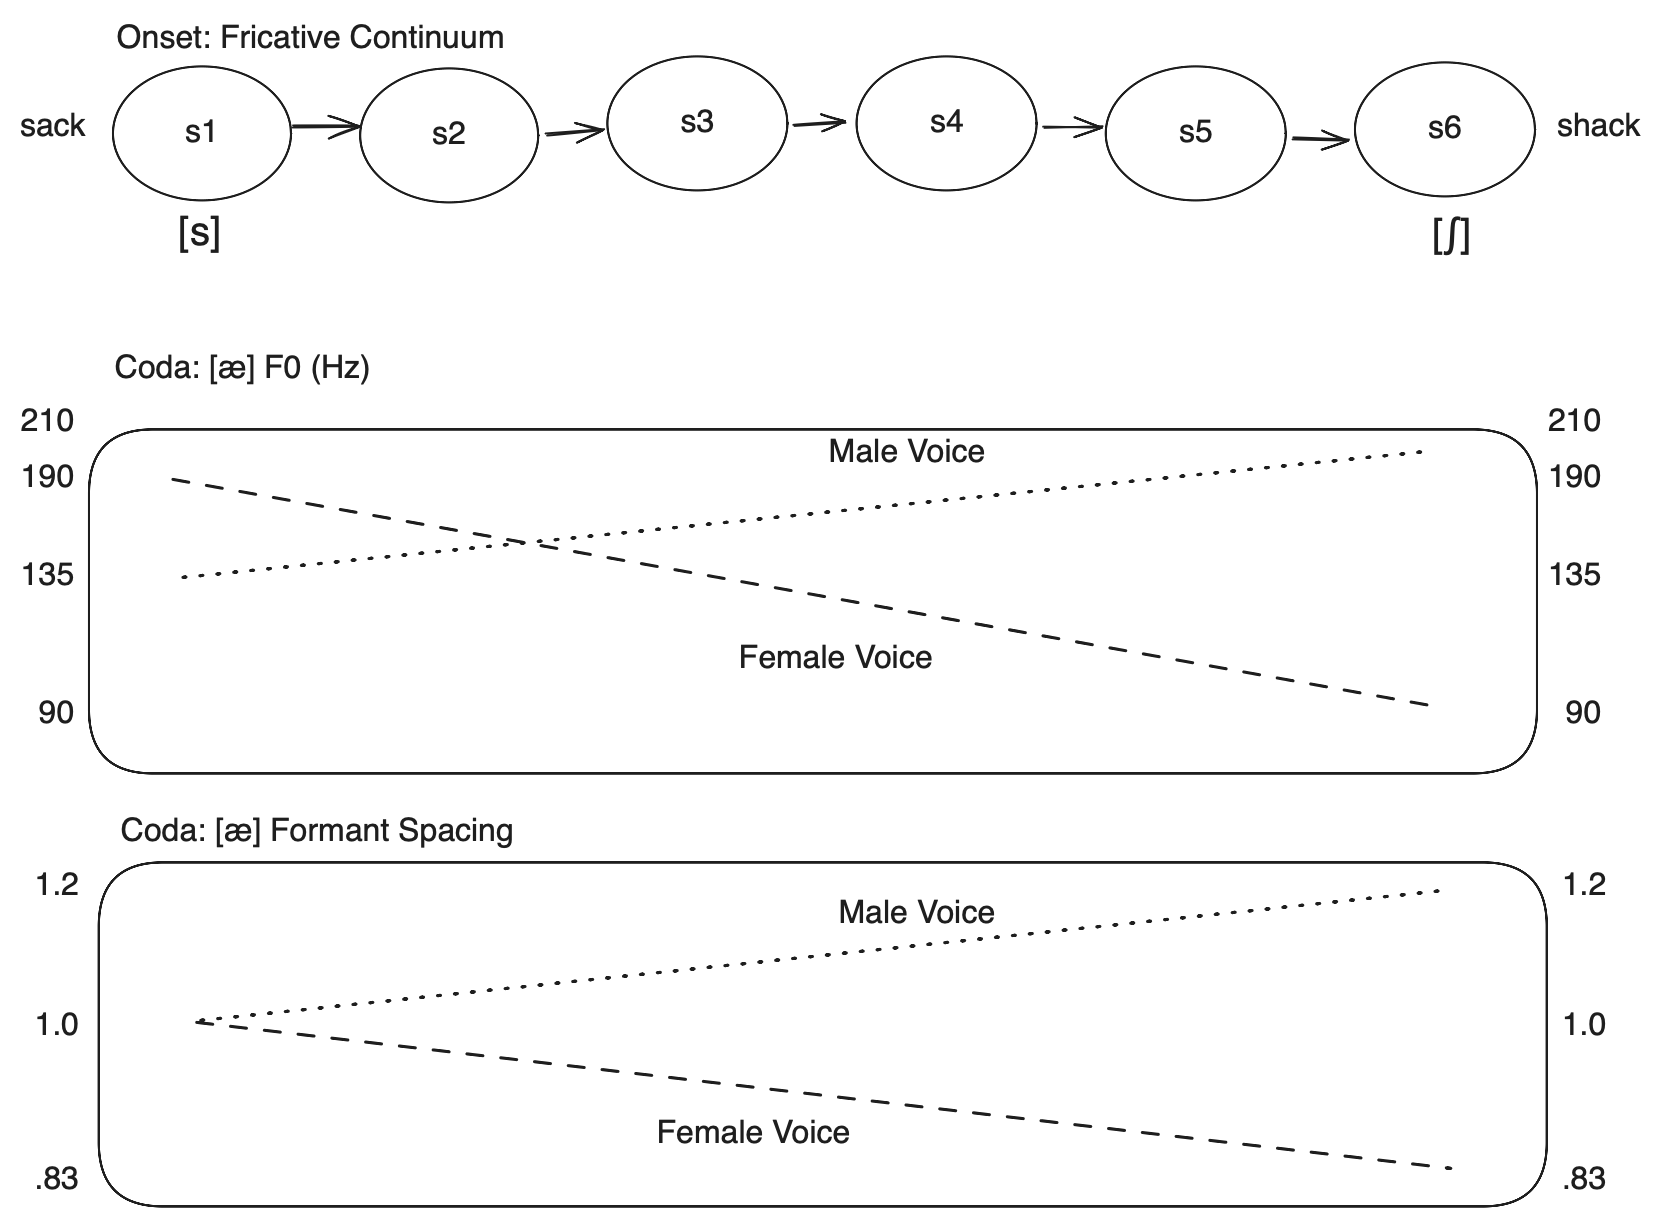
\includegraphics[width=0.8\linewidth,height=\textheight,keepaspectratio]{images/figure1.png}

}

\caption{\label{fig-stimuli}Bouavichith et al. (2019) auditory stimulus
continua. S1-S6 represent six continuum steps from most \emph{sack}-like
to most \emph{shack}-like fricatives. F0 and Formant spacing ratio plots
show the manipulations to the Male and Female voiced vowels across five
coda steps.}

\end{figure}%

\subsection{Explicit Evaluations of Auditory
Stimuli}\label{sec-stim-evals}

To better understand how the auditory stimuli might influence
participants' perceptions of the two talkers, we elicited social ratings
for each voice. 40 undergraduate students at the Ohio State University
(25 female, 15 male, ages 18-26) who participated in an in-person pilot
version of the experiment were asked to make judgements regarding the
gender, gender prototypicality, and sexuality of a natural,
unresynthesized production of \emph{sack} produced by each of the two
talkers. Participants listened to the recording and selected from a
fixed set of responses; no free form responses were elicited.

Participants' judgements of the female voice indicate general agreement
about this speaker's gender identity. Most participants (93\%) indicated
the speaker's gender to be female (2 participants specified
`trans-female'), and 3 were unsure or otherwise unable to determine. For
the female voice, average prototypicality ratings (in which, for a given
gender, 0 is least prototypical, and 5 is most prototypical) were 4.3/5
if the participant had indicated `female', and 2.75/5 if the participant
had specified `trans female'. Judgements of the voice's sexuality were
more variable, with 54\% indicating they were unsure, 40\% indicating
most likely heterosexual, and 1 participant each indicating most likely
bisexual or another sexuality.

Participants' judgements of the male voice suggest similar agreement.
80\% of participants indicated the speaker's gender to be male (1
specified `trans-male'), and 20\% were unsure. Average prototypicality
ratings were lower for the male speaker but similarly consistent: 3.6/5
if the participant had indicated the voice belonged to a `male' speaker,
and 2/5 if they had indicated the person speaking was a `trans male'. As
with the female voice, judgements of the voice's sexuality were more
variable. 65\% indicated they were unsure, 14\% indicated most likely
heterosexual, and 16\% indicated homosexual, and, again, 1 each
indicating most likely bisexual or another sexuality not listed.
Importantly, no participants rated the female voice as male or the male
voice as female. The variation among ratings is likely due to the
presentation of options beyond binary female and male categories and/or
to the current cultural understanding of gender performance as distinct
from sex. Despite this variability in responses, no `implausible'
answers were given. All things being equal, it is reasonable for a
listener to believe there may be little perceptual difference in cis and
trans voices for either male or female performances (Zimman, 2018), and
reasonable to consider `unsure' the most acceptable option in lieu of
asking the talker for their gender identity.

\subsubsection{Visual Stimuli}\label{sec-stimuli-visual}

The visual stimuli used in this study, again identical to the images
used in Bouavichith et al. (2019), are shown in Figure~\ref{fig-visual}.
These included two face images used for the guise manipulation, which
were retrieved from the Chicago Face Database (Ma et al., 2015), a
resource containing high-resolution, normed images of faces indexed by
gender and ethnicity. The faces selected were normalized for both
physical attributes (i.e., measurements of particular facial
dimensions), subjective ratings such as attractiveness, and for gender
and gender prototypicality. As in Bouavichith et al., CFD-WF-015-006-N
was selected as the representation of the gender-protypical female
talker and CFD-WM-029-023-N was selected as the representation of the
gender-prototypical male talker. Both images were converted to
greyscale.

Additionally, two greyscale line drawings were used as visual
representations of \emph{shack} and \emph{sack}. These images were used
in place of orthographic targets to maintain consistency with
Bouavichith et al's design and to facilitate future eye tracking
investigation of this phenomenon. This is a divergence from the original
Strand \& Johnson design, which represented target words
orthographically.

\begin{figure}

\centering{

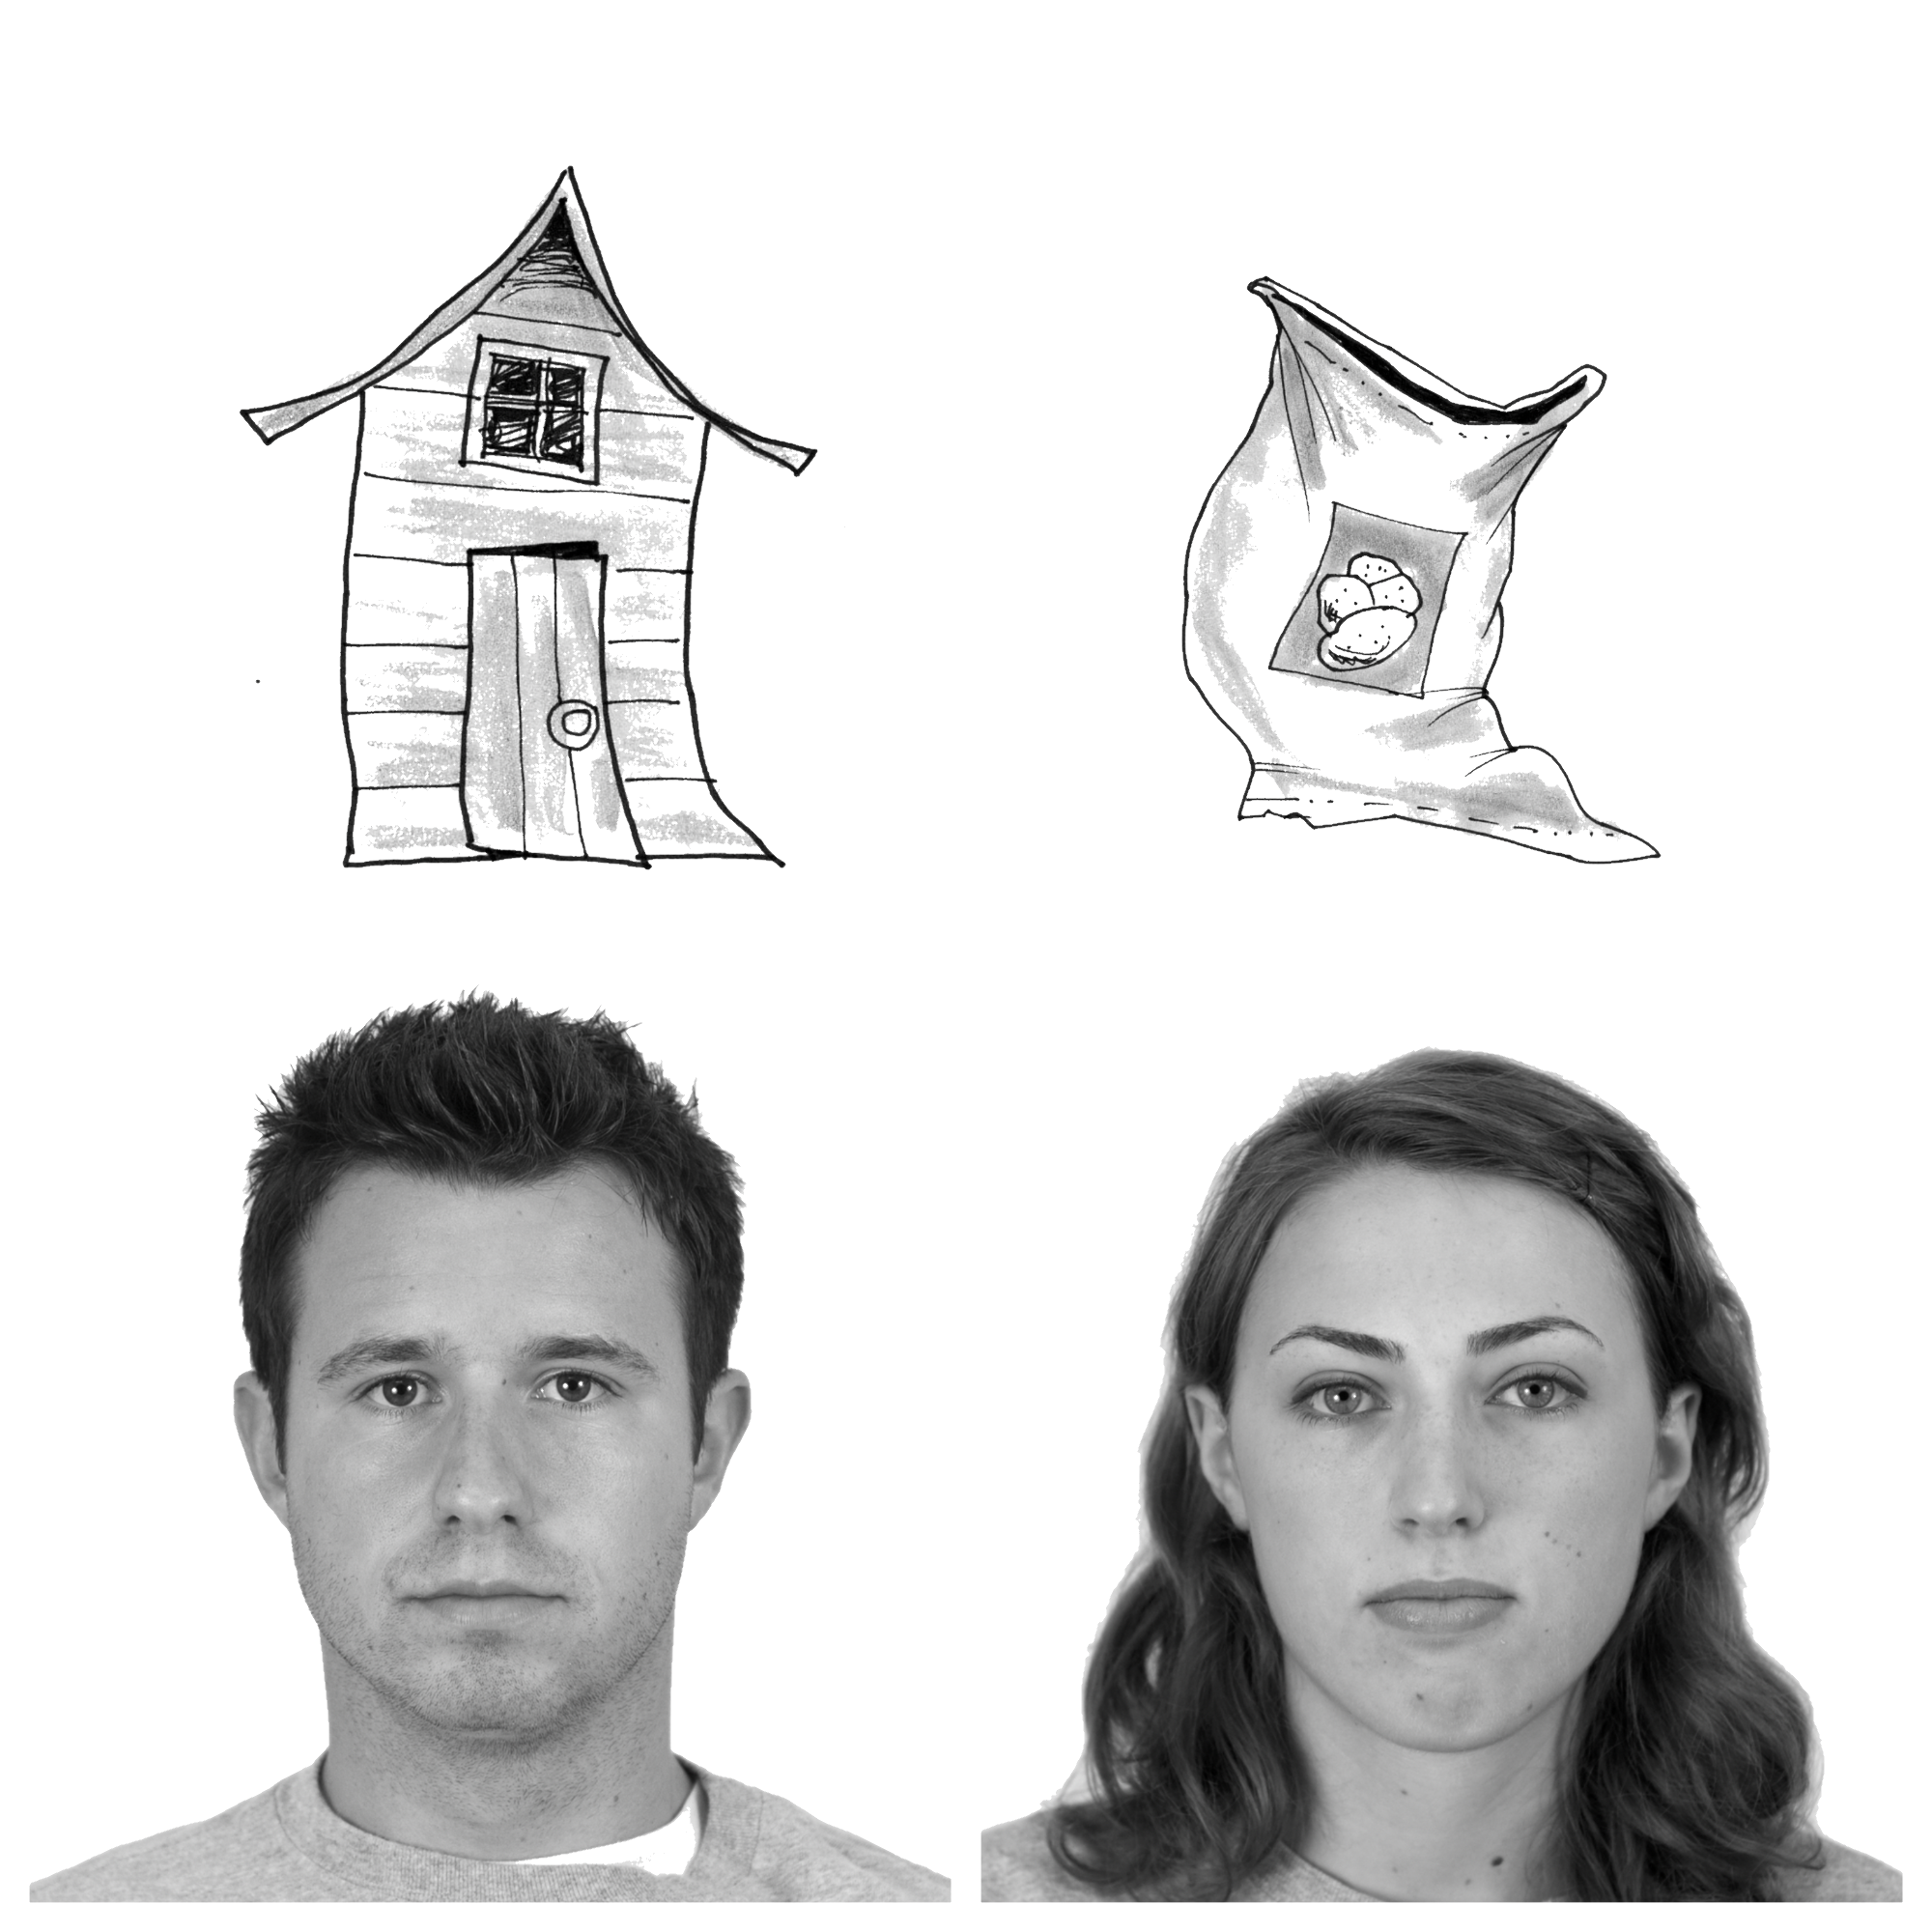
\includegraphics[width=0.8\linewidth,height=\textheight,keepaspectratio]{images/facesanddrawings.jpg}

}

\caption{\label{fig-visual}Stimuli comprised \emph{shack} and
\emph{sack} targets (top) and gender-protypical `male' and `female'
faces (bottom)}

\end{figure}%

\subsection{Procedure}\label{sec-procedure}

The experiment was created in OpenSesame v3.3 (Mathôt et al., 2012) and
exported for the web using OSWeb v1.4.14.0. Modifications to the
experiment included translating portions of the Python code into
JavaScript and adding code to collect Prolific IDs and provide proof of
completion to Prolific. This experiment was hosted on a JATOS (Lange et
al., 2015) instance on an Ohio State University Linguistics Department
server. Participants received a link to the experiment via Prolific and
used their own computers, keyboards, and headphones to complete the
experiment.

Participants were randomly assigned to one of two between-subjects
awareness conditions. These conditions differed only in the initial
information provided as to the nature of the experiment. Participants in
the \emph{hidden} condition experienced a standard Matched Guise task.
They were given no information about the task or the stimulus materials
beyond the general instructions for completing the experiment: listen to
the voice, press `z' if you heard the word on the left, press `m' for
the word on the right. Participants in the \emph{unhidden} condition
also received this instruction, but were given a partial debriefing
regarding the task. They were informed that-- while they would see faces
onscreen while hearing words-- the voices in a given trial were not
produced by the person shown in the images; the images had been
downloaded from a database of photographs created for experimental use,
and that the auditory and visual stimuli were in no way related to each
other. Participants were divided equally among these two conditions.
Neither awareness condition was informed about the synthetic nature of
the auditory stimuli.

Participants were also assigned to one of two gender congruity
conditions. Although the manipulated rimes sounded gender ambiguous to
us and had been rated as ambiguous by pilot participants in Bouavichith
et al. (2019), the possibility remained that the voices, particularly at
the endpoints, might be perceived incongruously with the faces (McGowan,
2015)\footnote{We use `congruous' and `incongruous' (Schulman, 1974)
  intentionally to suggest faces and voices may pattern together in
  particular ways in listeners' experience with no implied claim that
  voices may `match' or `mismatch' in some intrinsic way.}.

In congruous trials, the faces and voices were paired such that
participants were only presented with auditory stimuli from the female
talker's continuum alongside the female face, and tokens from the male
talker were only presented alongside the male face. In incongruous
trials, by contrast, auditory stimuli from the female talker's continuum
were only ever presented alongside the male face, and tokens from the
male talker's continuum were only ever presented alongside the female
face. Half of participants were randomly assigned to each congruity
condition, resulting in a 4-way between-subjects design across
instruction and congruity conditions. Each participant heard all 60
auditory stimuli; 30 paired with the male face and 30 paired with the
female face.

In each trial, participants were shown one of the two faces for 1500 ms.
Following this initial presentation, the face remained onscreen and was
flanked by the \emph{shack} and \emph{sack} images. Simultaneously, one
of the auditory stimuli was played over the headphones. The trial ended
when the participant pressed an appropriate key on their physical
keyboard, and their response and reaction time data were uploaded to the
JATOS instance. In both congruous and incongruous conditions, all 60
unique trials (30 per face) were presented twice to each participant for
a total of 120 trials.

\section{Predicted Results}\label{sec-predictions}

\subsection{Face: male or female}\label{sec-pred-face}

Consistent with previous results, when face and voice provide congruent
social information, we anticipate that more of the {[}ʃ{]}-{[}s{]}
continuum will be heard as {[}ʃ{]} when participants are shown the
female face and more to be heard as {[}s{]} when participants are shown
the male face.

\subsection{Congruence: pairing of face and
voice}\label{sec-pred-congruence}

However, when face and voice provide incongruent social information, we
do not expect to replicate this shift in fricative category boundary. To
our knowledge, the influence of incongruence has not been directly
investigated for listeners' joint perception of gender and fricative
place. Johnson et al. (1999) tests AV integration of Male and Female
faces with prototypical and non-prototypical gendered voices in a vowel
quality perception task. They find what may be an incongruence effect
with the prototypical male voice; listeners reported no difference in
perceived vowel quality with this voice in either Face condition
(Johnson et al., 1999, p. 376). We expect incongruity to influence
perception for both voices, but the effect may be stronger with a
prototypically male voice (King, 2021).

We make a similar prediction for reaction times. Johnson et al. (1999)
did not collect reaction time data, and McGowan (2011) reports
inconsistent reaction times for incongruous trials across different
tasks. However, Whalen (1984) finds that listeners judgements are slowed
by coarticulatory mismatches. If coarticulatory and social variation are
processed similarly, this should hold for listeners' identification of
fricatives on a {[}ʃ{]}-{[}s{]} continuum. Therefore, we predict longer
reaction times for Incongruous conditions. Furthermore, when gender
information is most clear, at gender continuum steps 1 and 2 for the
Male talker and at gender steps 4 \& 5 for the Female talker, and in
conflict with the presented Face, listeners' response times should be
slowest.

Since strong phonetic correlates of gender, pitch and formant spacing,
have been manipulated over the course of the VC rime continua in our
auditory stimuli, we anticipate that the nullifying effect of
incongruous face and voice on fricative perception should be strongest
for the natural end points of the continua where the difference is most
salient and should weaken as phonetically-cued gender information
becomes more ambiguous. These stimuli have been independently normed for
ambiguity (Bouavichith et al., 2019, p. 1040) in the 2nd and 3rd levels
of the rime continua. This means we anticipate an interaction between
Face and Rime step but only in the incongruous trials and only at the
extremes of the rime continuum.

\subsection{Guise: Hidden or Unhidden}\label{sec-pred-guise}

The care researchers take to ensure that the guise manipulation is
hidden from participants suggests a kind of imagined fragility of the
effects of social information on language perception. From this view:
listeners who become aware of the guise manipulation will have
introspective access to and deliberative control over the influence of
visual social information on perception. If this is true, explaining the
guise manipulation, in the unhidden condition, should have a strongly
negative effect on the Strand effect. Alternatively, if the influence of
social information on fricative perception is not available to
introspection or deliberative control, we should see no change between
the hidden and unhidden conditions.

Additionally, we speculate that there may be a response time difference
between the Hidden and Unhidden guises even if there is no apparent
difference in percept between the conditions. It may be the case that
participants will arrive at the same behavioral responses via different
cognitive processing paths, perhaps drawing on different levels of
knowledge and awareness, and that these differences may be detectable in
response times between the Instruction conditions.

\section{Results}\label{sec-results}

Participants provided a total of 14,400 trials (120 trials from each of
120 online participants; 3600 trials in each instruction x congruity
condition). It is not clear what it means to be `accurate' when asked to
perceive fricatives from a continuum, so accuracy was calculated only
for responses to the {[}ʃ{]} and {[}s{]} endpoints. Overall,
participants were highly accurate (96.8\%) but four participants were
excluded from further analysis for accuracy below the predetermined 85\%
threshold reducing the total number of trials to 13,920. Trials were
coded as correct if the participant responded `shack' to onset step 1 or
`sack' to onset step 6. The four excluded participants all scored 67.5\%
accuracy or lower.

An additional 50 trials were excluded due to response times that were
either too fast or too slow. To reduce the effects of response time
outliers on subsequent analyses, all response times shorter than 50 ms
(N=0) and longer than 5000 ms (N=50) were excluded. The 5000 ms response
time cutoff was used instead of imposing an in-experiment time limit on
responses to a trial to ensure that participants were required to
respond to each trial. Altogether, 530 trials were excluded, leaving
data from 13,870 trials for analysis (approximately 96.3\% of the
initial data set). The majority (96.8\%) of the remaining response times
were within a range between 200 and 2000 ms. To increase normality of
the distribution of response times across participants, the remaining
response times were log-transformed.

\subsection{{[}ʃ{]}-{[}s{]} Percepts}\label{sec-results-fricative}

Figure~\ref{fig-scurve} presents listeners' percepts on this 2AFC task.
The horizontal axis in each of these four plots is the fricative
(syllable Onset) continuum step. Step 1 of the continuum is most
{[}ʃ{]}-like, step 6 is the most {[}s{]}-like, steps 3 \& 4 are the most
ambiguous. Darker lines in Figure~\ref{fig-scurve} present trials using
the female Face; lighter lines present trials using the male Face. The
Hidden and Unhidden instruction conditions are represented by the left
and right columns of figures, respectively. The rows present the
Congruous blocks where Face and Coda speaker voice shared a gender
identity (top) and Incongruous trials where Face and Coda speaker voice
mismatched in gender identity (bottom).

\begin{figure}

\centering{

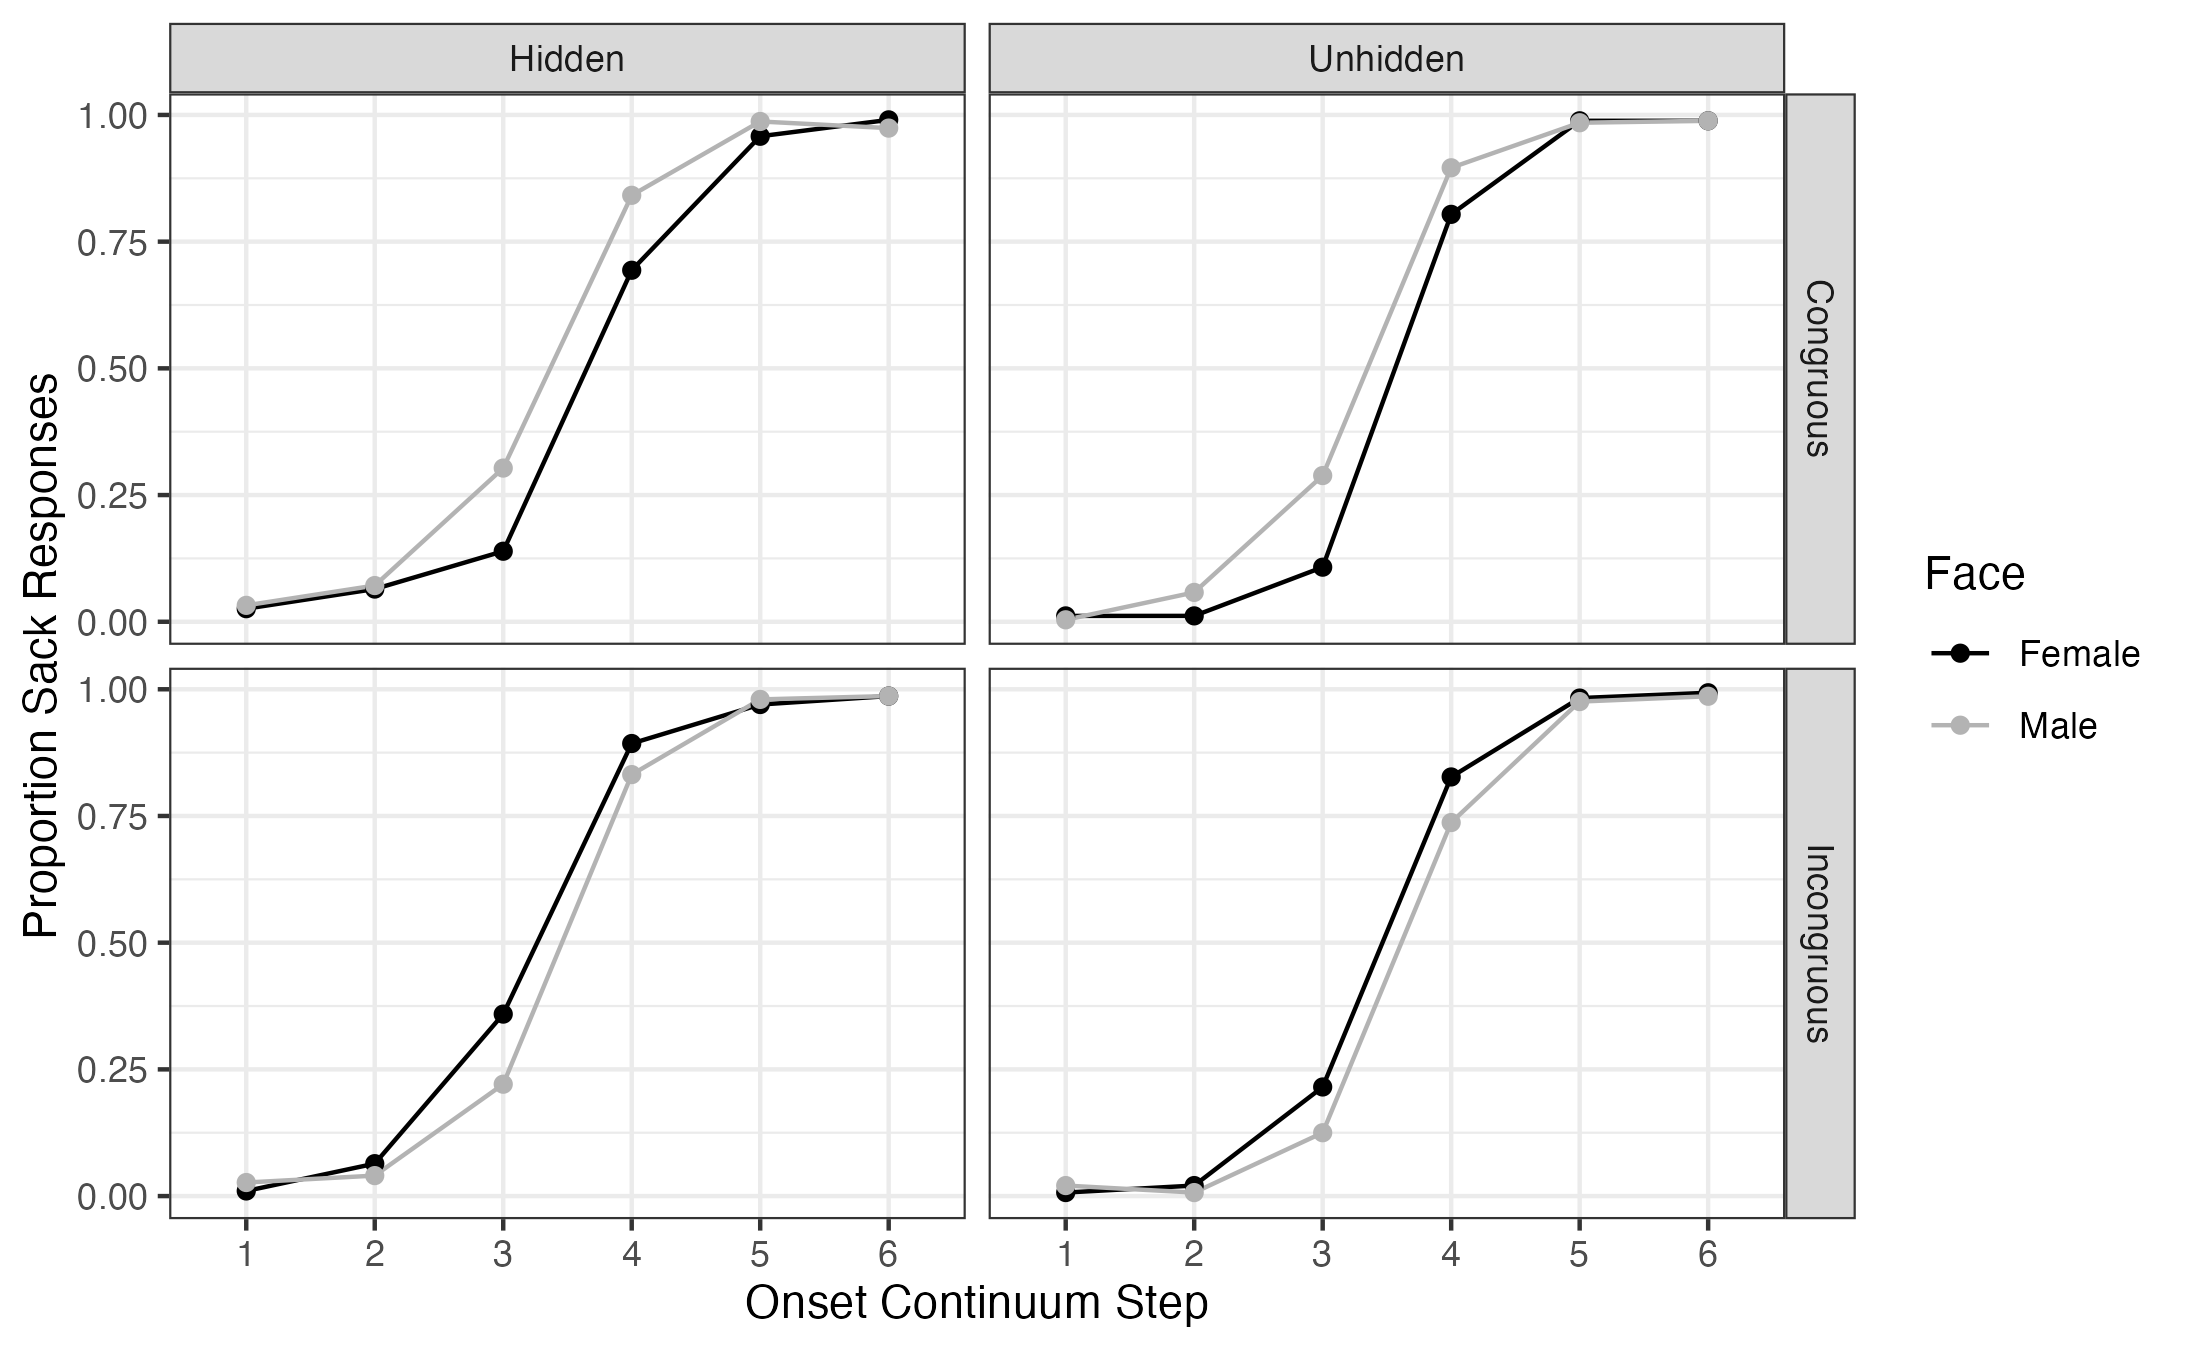
\includegraphics[width=0.8\linewidth,height=\textheight,keepaspectratio]{images/Scurve.png}

}

\caption{\label{fig-scurve}\emph{sack} responses plotted as a function
of {[}ʃ{]}-{[}s{]} onset continuum steps and purported gender of the
face.}

\end{figure}%

A successful replication of the Strand effect would mean that a higher
proportion of the ambiguous stimuli would be heard as {[}s{]} when the
purported gender suggested by the face is male than when the face is
female. This pattern appears to hold in both the Hidden and Unhidden
conditions, but only when gender identity of the talker who produced the
CV rime stimuli was congruous with the gender presented in the visual
portion of the guise. From Figure~\ref{fig-scurve} it would appear that
listeners' reported percepts more closely track the voice of the talker
than the face in the picture when these sources of information are
incongruous.

\begin{figure}

\centering{

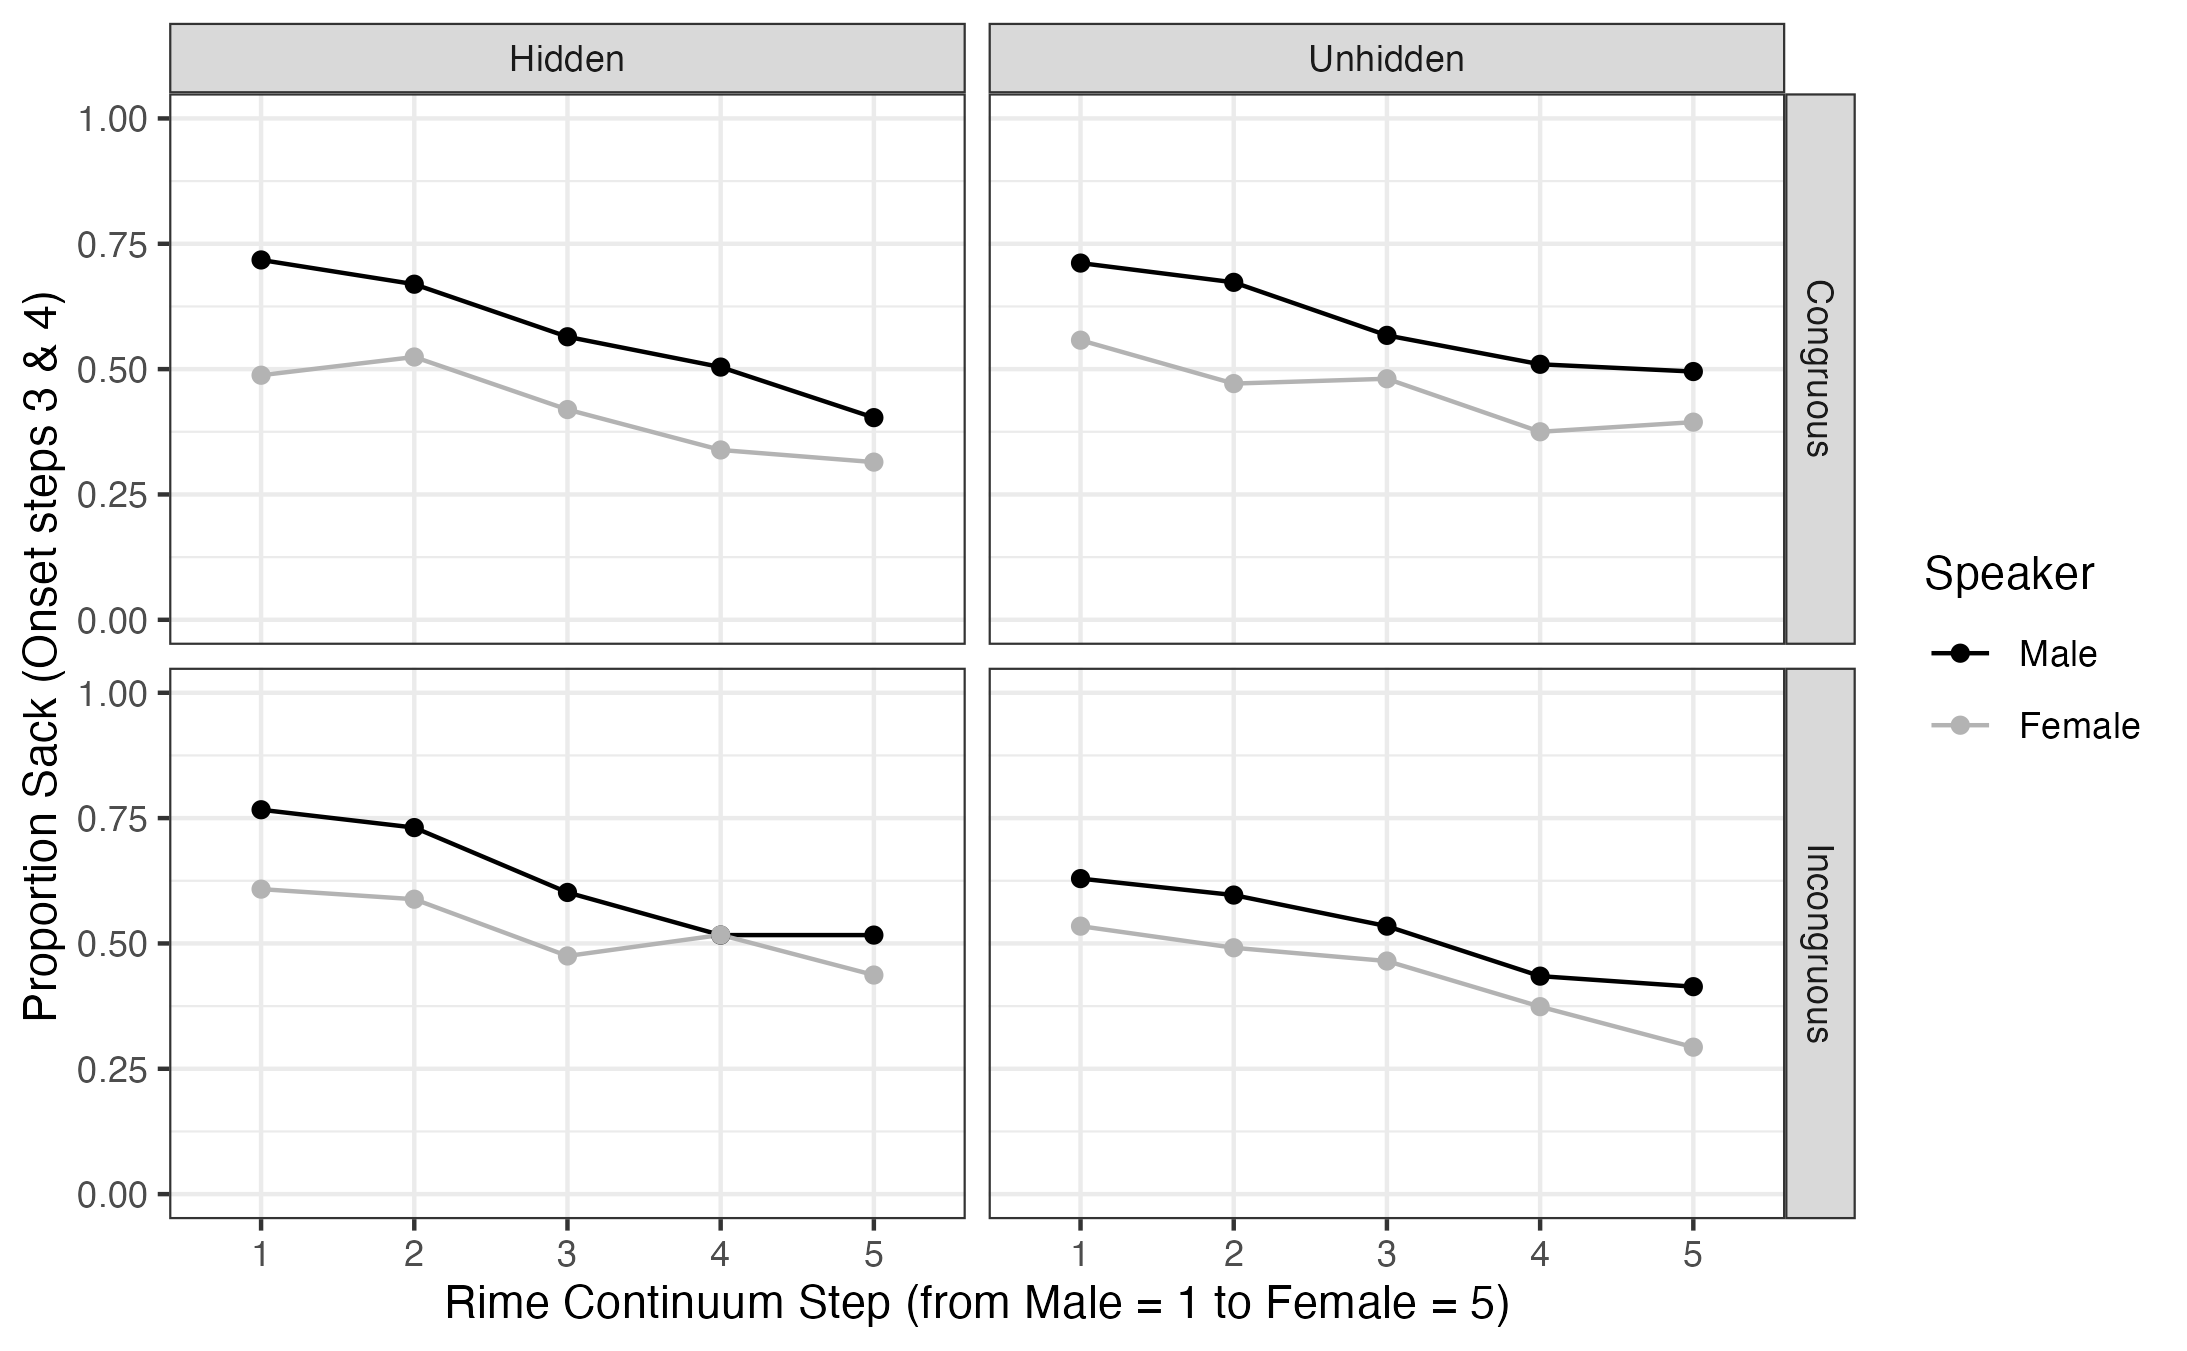
\includegraphics[width=0.8\linewidth,height=\textheight,keepaspectratio]{images/ambiguous-by-rime-step.png}

}

\caption{\label{fig-rimes}`sack' responses to ambiguous fricative trials
plotted as a function of CV rime continuum steps and gender of stimulus
talker.}

\end{figure}%

Given that our stimuli included manipulations of F0 and formant spacing
to modify the gender typicality of the male-provided and female-provided
recordings, one might expect that the results in Figure~\ref{fig-scurve}
might represent only listener responses to the original, unmodified
stimuli, but this is not the case. These four subplots include fricative
responses across the entire rime continuum. However, this does not mean
the resynthesis was entirely unsuccessful. We predicted that, since
these phonetic correlates of gender have been manipulated over the
course of the VC rime continua, the effect of incongruence should be
strongest for the end points of the continua where the social
information presented by the voice is, presumably, most salient and
weaker as phonetically-cued gender information becomes more ambiguous.
Figure~\ref{fig-rimes} suggests this prediction is at least partially
borne out. Figure~\ref{fig-rimes} plots proportion `sack' responses to
the ambiguous portion of the {[}ʃ{]}-{[}s{]} continuum (steps 3 \& 4) as
a function of rime continuum step. The lines plot Speaker, rather than
Face, and the meaning of line color has changed in this figure: dark
lines represent responses to stimuli originally produced by the male
talker and the lighter lines represent responses to stimuli originally
produced by the female talker. Step 1 on this continuum, in each of the
four subplots, includes the most natural token for the male talker and
the most manipulated token for the female talker while step 5 includes
the most natural token for the male talker and the most manipulated
token for the female talker. As before, columns present the Hidden and
Unhidden conditions while rows present the Congruous and Incongruous
blocks.

In a 2AFC task with unbiased stimuli, chance is 50\%. Responses at the
.5 line in Figure~\ref{fig-rimes} suggest that the ambiguous fricatives
remained ambiguous, while responses that tend to be above this line
reflect a tendency toward {[}s{]} percepts and responses that tend to be
below this line reflect a tendency toward {[}ʃ{]}. Across all 4
conditions, we observe a declination from highest-proportion {[}s{]}
responses in step 1 of the F0 continua to lowest in step 5. When face
and voice were congruous, virtually all male-voice (and male face)
responses are above or at 50\% `sack' and virtually all female-voiced
(and female face) responses are at or \emph{below} 50\% `sack'. This is
the same pattern that can be observed at Onset continuum steps 3 \& 4 in
Figure~\ref{fig-scurve}. It is not clear from Figure~\ref{fig-rimes}
alone if there is any difference between the Congruous and Incongruous
conditions. However, it is important to recall about the bottom row of
this figure that male talker responses in the incongruous trials were
presented with a female face while female talker trials were presented
with a male face. Even a weakly-significant Strand effect would predict
that the female talker, particularly on the more ambiguous continuum
steps, should show more `sack' responses consistent with having been
shown a male face and no such effect is evident in this plot.

Indeed, a striking feature of these figures
(\ref{fig-scurve}, \ref{fig-rimes}) is how the apparent influence of
gender information flips between congruous and incongruous conditions in
the former but remains essentially constant in the latter. Taken
together, these plots suggest that cues to gender in the voice are a
stronger predictor of listeners' reported percept in this matched guise
task than just the purported gender of the face but that, while
manipulations of F0 and formant spacing may shift the gender
\emph{typicality} of a prototypical female or male voice at this low,
segmental level.

The main objective of this experiment was to explore the role of
listener awareness in the matched guise technique. Here again the
overall trend is clear: if there is an effect of explaining to
participants that the voice and face in the matched guise task are
unrelated to each other, that effect is so weak as to be essentially
invisible in these visual interrogations of the data. Categorical
responses in the Hidden and Unhidden instruction conditions appear to be
identical.

\subsection{Logistic Regression and Quantitative
Analysis}\label{sec-results-stats}

These qualitative assessments of listener responses can be examined
further through quantitative analysis. Through model comparison, we
arrived at a logistic mixed model to predict percept with Congruity
condition, instruction condition, Onset step, Face, and Rime step with
interactions for all but Rime step. This model was justified by model
selection but given the notorious difficulty of interpreting a 4-way
interaction and the preceding visual inspection of the data, we opted to
separate Congruence into a pair of 3-way models. Using \texttt{glmer()}
(Bates et al., 2011), we divided the data into congruous and incongruous
subsets and fitted a pair of logistic mixed models (estimated using ML
and BOBYQA optimizer) to predict percept with Instruction condition,
Onset.step, Face and Rime.step
(\texttt{percept\ \textasciitilde{}\ Instruction\ *\ Onset.step\ *\ Face\ +\ Rime.step}).
The models included random intercepts for subject. All categorical
predictors were coded using contrast coding.

\begin{figure}

\centering{

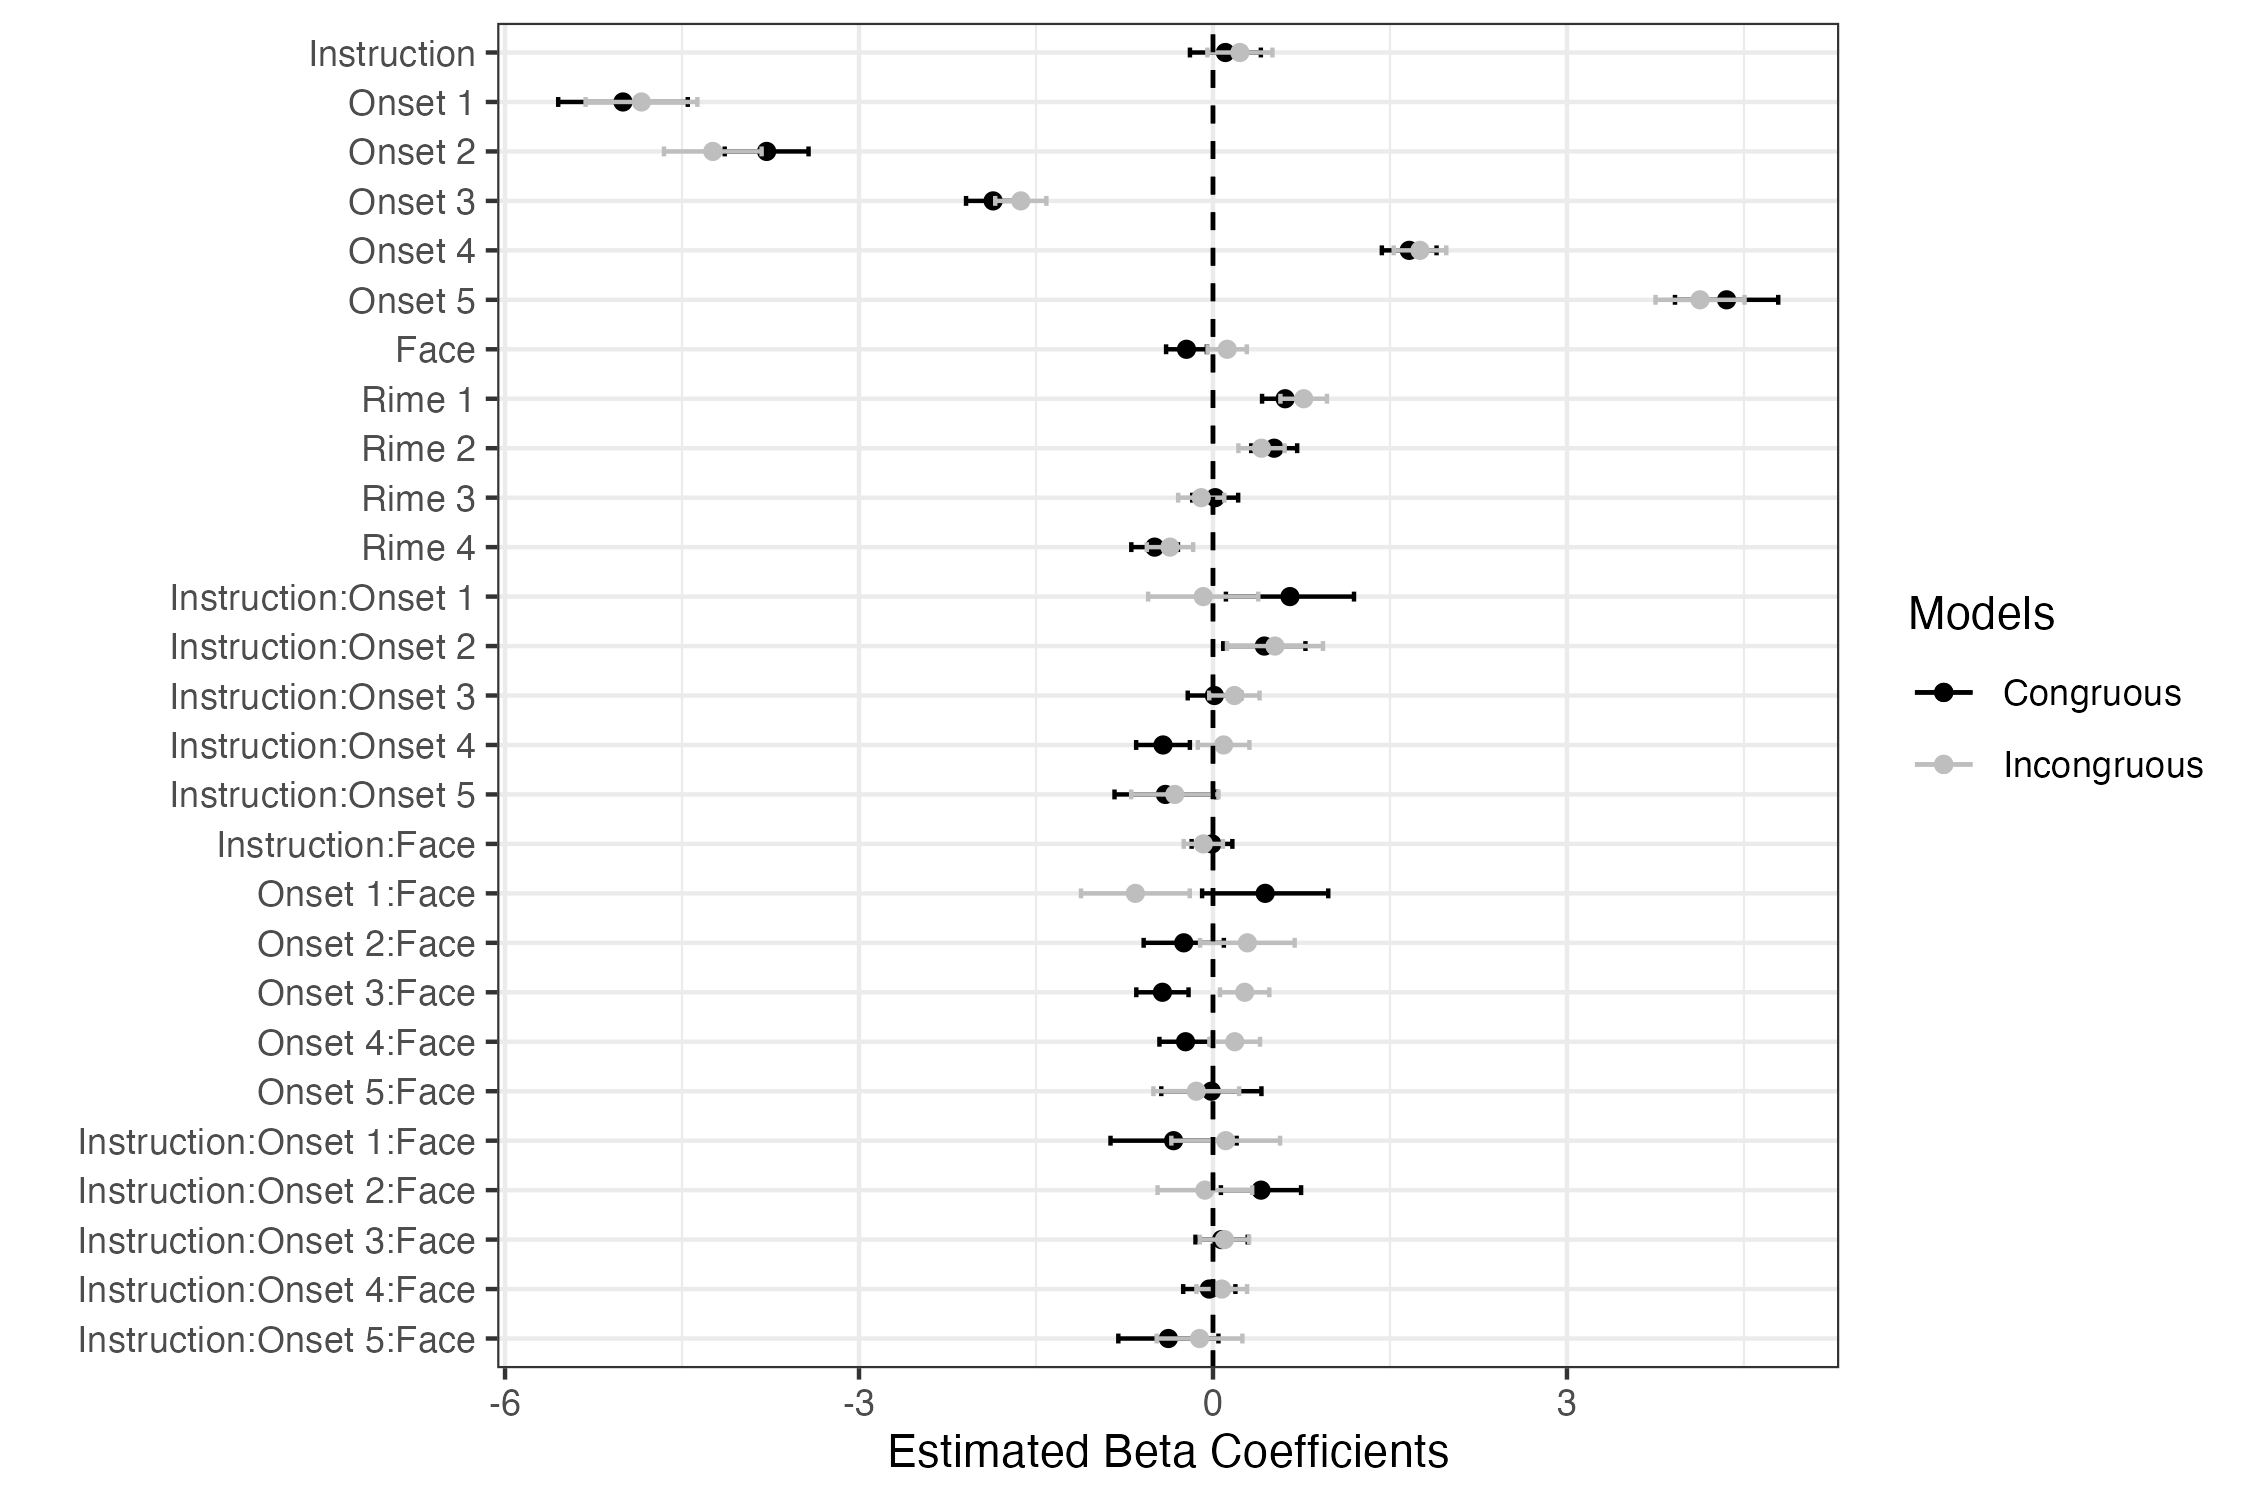
\includegraphics[width=0.8\linewidth,height=\textheight,keepaspectratio]{images/coefs_instruction.png}

}

\caption{\label{fig-coefs}Beta coefficients for responses in the
Congruous (black) and Incongruous (gray) logistic regression models
plotted with 95\% confidence intervals.}

\end{figure}%

Beta coefficients for the two separate logistic mixed models are plotted
together in Figure~\ref{fig-coefs}. Terms plotted to the left of the
dashed zero line have a negative influence on `sack' percepts in the
model, while terms plotted to the right have a positive influence. As a
consistency check, we can observe that the levels of the Onset continuum
behave in precisely the expected ways and all levels are statistically
significant predictors of percept in both models. Onset step 1 ({[}ʃ{]})
is negatively associated with `sack' responses and significant in both
the Congruous (\(β=-5.00\), \(SE=0.28\), \(p < 0.001\)) and Incongruous
(\(β=-4.84\), \(SE=0.24\), \(p < 0.001\)) models. Onset step 5 ({[}s{]})
is positively associated with `sack' responses and significant in both
the Congruous (\(β=4.35\), \(SE=0.22\), \(p < 0.001\)) and Incongruous
(\(β=4.12\), \(SE=0.19\), \(p < 0.001\)) models.

As visual inspection of the data suggests, this study includes a
replication of the Strand effect in the Congruous condition. There is a
main effect of Face in the model (\(β=-0.22, SE=0.09, p<0.05\)). Face is
negatively associated with `sack' responses suggesting that, with these
stimuli, at least, it is more appropriate to understand the effect of
Face as an increase of `shack' responses given the female Face. The
inclusion of the interaction term for Onset and Face allows us to see
that the effect of Face is greatest on the ambiguous Onset steps 3
(\(β=-0.43\), \(SE=0.11\), \(p < 0.001\)) and, to a lesser extent, 4
(\(β=-0.23\), \(SE=0.11\), \(p < 0.05\)).

However, the Strand effect observed in the Congruous condition is not
attributable entirely to the main effect of Face. Rime F0 is also
significant; Rime level 1, the male end of the continuum, is positively
associated with `sack' responses (\(β=0.61\), \(SE=0.10\),
\(p < 0.001\)) as is Rime level 2 (\(β=0.52\), \(SE=0.10\),
\(p < 0.001\)). Rime level 3, where the continuum is most gender
ambiguous, is not statistically significant. Rime level 4, on the female
end of the continuum, is negatively associated with `sack' responses and
significant (\(β=-0.49\), \(SE=0.10\), \(p < 0.001\)).

We can confirm that the Strand effect has not been replicated in the
Incongruous condition. As is visible in the bottom row of
Figure~\ref{fig-scurve}, the effect of Face on `sack' responses is not
significant. The interaction of Onset and Face also behaves quite
differently in the Incongruous model. Onset x Face is negatively
associated with `sack' responses at Onset step 1 (\(β=-0.66\),
\(SE=0.24\), \(p < 0.001\)) but positively associated with `sack'
responses and significant at Onset step 3 (\(β=0.27\), \(SE=0.11\),
\(p < 0.05\)).

Interestingly, the significant effect of Rime observed in the Congruous
model also holds, nearly identically, in the Incongruous model. Rime
level 1, the male end of the continuum, is again positively associated
with `sack' responses (\(β=0.77\), \(SE=0.10\), \(p < 0.001\)) as is
Rime level 2 (\(β=0.41\), \(SE=0.10\), \(p < 0.001\)). Rime level 3 is
also not statistically significant in the Incongruous model. Rime level
4, on the female end of the continuum, is negatively associated with
`sack' responses and significant (\(β=-0.36\), \(SE=0.10\),
\(p < 0.001\)).

Finally, the quantitative analysis exploring the effect of unhiding the
matched guise manipulation from participants largely supports the
qualitative analysis. As can be observed in Figure~\ref{fig-coefs},
there is no significant main effect of Instruction condition in either
model. Still, a somewhat more nuanced picture emerges from the
interactions of Instruction condition with Onset and the 3 way
interaction of Instruction, Onset, and Face in the Congruous trials. The
interaction of Instruction with Onset is significant, or nearly so, at
every step of the fricative continuum other than the most significant.
In the {[}ʃ{]}-like portion of the continuum, the interaction with face
is positively associated with `sack' responses at step 1 (\(β=0.65\),
\(SE=0.28\), \(p < 0.05\)) and 2 (\(β=0.44\), \(SE=0.18\),
\(p < 0.05\)). The interaction of guise with the most ambiguous onset
step is not significant (\(β=0.011\), \(SE=0.12\)). The interaction of
Instruction with Onset step 4, on the {[}s{]} end of the continuum is
negatively associated with `sack' responses and statistically
significant (\(β=-0.43\), \(SE=0.12\), \(p < 0.001\)). Instruction x
Onset step4 is also negatively associated with `sack' responses but does
not reach significance at the standard alpha level (\(β=-0.40\),
\(SE=0.22\), \(p = 0.067\)). The 3-way interaction of Instruction x
Onset x Face is positively associated with `sack' responses at step 2
(\(β=0.41\), \(SE=0.17\), \(p < 0.05\)) and weakly, but not
significantly, negatively associated with `sack' responses at step 5
(\(β=-0.38\), \(SE=0.21\), \(p = 0.080\)).

There is also no main effect of Instruction in the Incongruous trials.
The 3-way interaction of Instruction x Onset x Face also does not reach
statistical significance. However the 2-way interaction of Instruction
with Onset step is positively associated with `sack' responses at Onset
step 2 (\(β=0.53\), \(SE=0.21\), \(p < 0.05\)) and approaches
significance at step 3, where it is weakly positively associated
(\(β=0.18\), \$SE=0.11, \(p = 0.095\)) and step 5 where it is weakly
negatively associated (\(β=-0.32\), \(SE=0.19\), \(p = 0.086\)).

\subsection{Response Times}\label{sec-results-rt}

We again opted to separate Congruence into a pair of 3-way models for
linear mixed model analysis of our log-transformed response time data.
Using \texttt{lmer()} (Bates et al., 2011), we reused the congruous and
incongruous subsets created for the logistic regression models and
fitted a linear mixed model (estimated using REML and nloptwrap
optimizer) to predict logRT with Guise, Onset, Face and Rime
(\texttt{logRT\ \textasciitilde{}\ Instruction\ *\ Onset\ *\ Face\ +\ Rime}).
The models included random intercepts for subject. All categorical
predictors were coded using contrast coding. Beta coefficients for both
models are plotted in Figure~\ref{fig-coefs-logRT}. Terms plotted to the
left of the zero line are associated with a decrease in log response
time while terms plotted to the right of the zero line are associated
with an increase in log response time. Notably, the longest response
times are associated with the most ambiguous steps of the
{[}ʃ{]}-{[}s{]} onset continuum. Onset step 3 is positively associated
with response time and significant in both the congruous (\(β=0.08\),
\(SE=0.007\), \(p < 0.001\)) and incongruous (\$β=0.0\$7, \(SE=0.007\),
\(p < 0.001\) ) models. The same is true of step 4 in the congruous
(\(β=0.07\), \(SE=0.007\), \(p < 0.001\)) and incongruous (\(β=0.07\),
\(SE=0.007\), \(p < 0.001\)) models as well. On the other hand, steps 1,
2, and 5 are all negatively associated with response time and also
significant in both models (see Figure~\ref{fig-coefs-logRT}).

\begin{figure}

\centering{

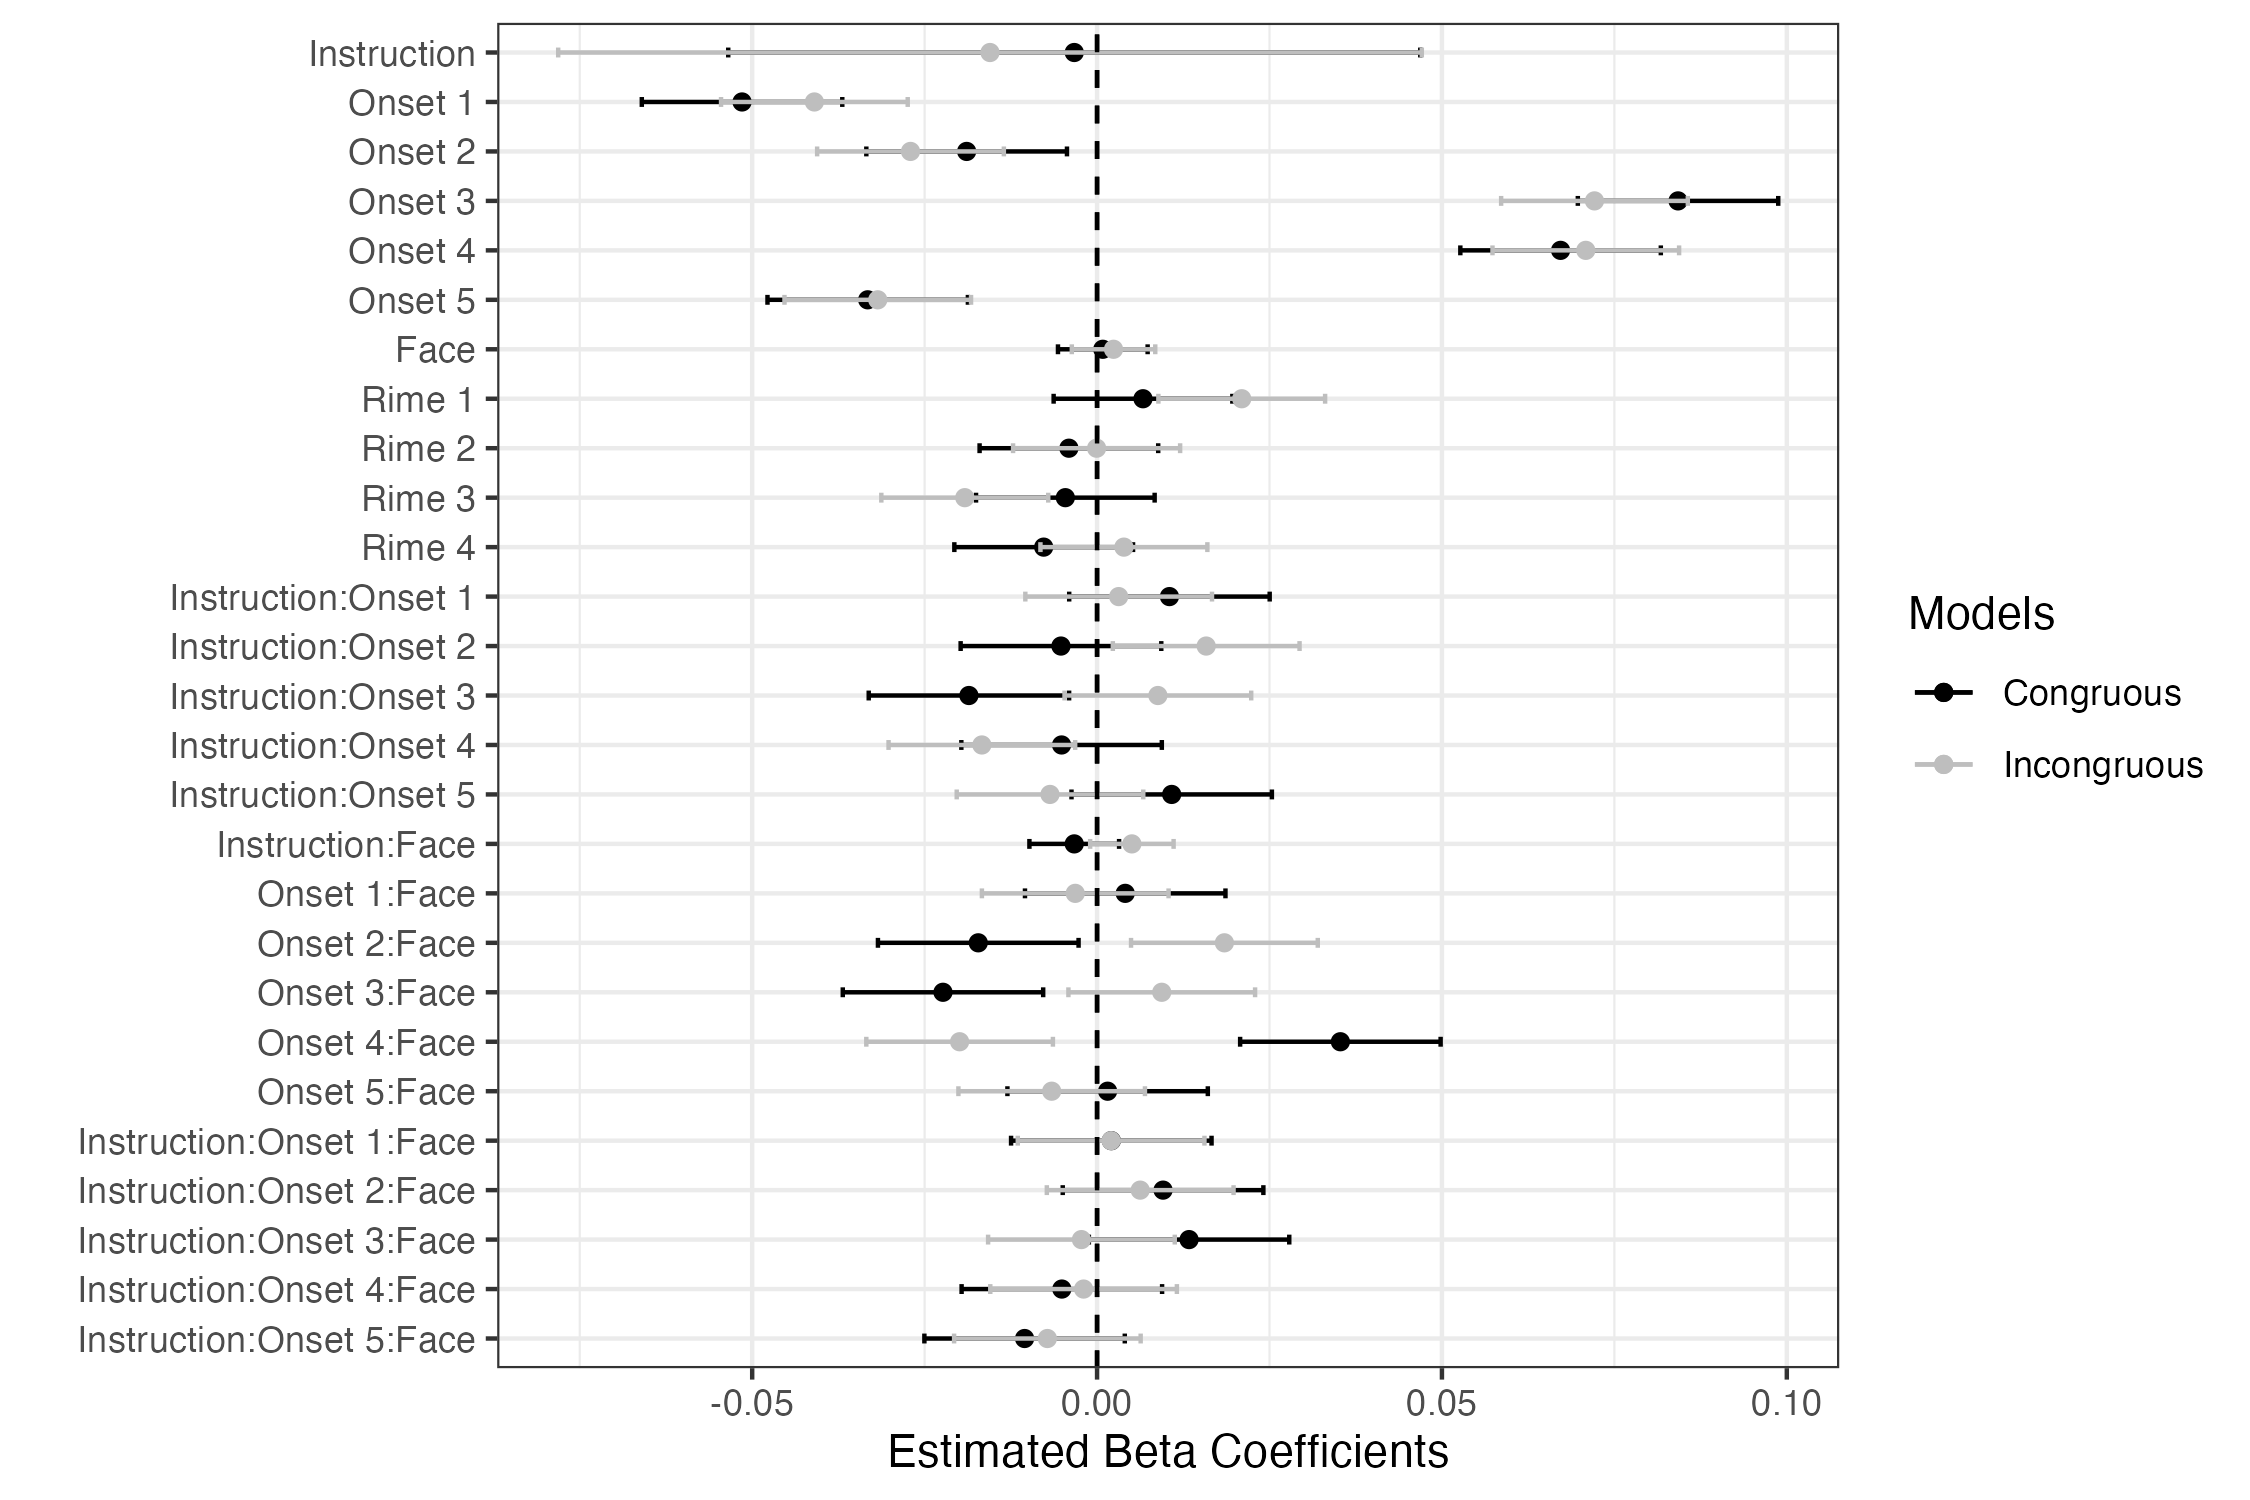
\includegraphics[width=0.8\linewidth,height=\textheight,keepaspectratio]{images/coefs-logRT_instructions.png}

}

\caption{\label{fig-coefs-logRT}Beta coefficients for log-transformed
response times in Congruous (black) and Incongruous (gray) linear
regression models plotted with 95\% confidence intervals.}

\end{figure}%

We predicted overall slower response times in the Incongruous than
Congruous conditions, but this prediction is not borne out by the data.
Apart from generally higher variability in the incongruous conditions,
there is no positive or negative trend in response times between the two
Congruity models. For example, within the Incongruous model response
times given the interaction of Onset step 3 * Face are longer
(\(β=-0.009\), \(SE=0.007\), \(p = 0.17\)), which would seem to support
our prediction, but response times for Onset step 4 * Face are shorter
(\(β-0.02\), \(SE=0.007\), \(p < 0.01\)), the opposite of what we
predicted. The exact opposite pattern appears within the Congruous model
where response times are shorter given Onset 3 * Face (\(β=-0.02\),
\(SE=0.007\), \(p < 0.01\)) but longer given Onset step 4 * Face
(\(β=0.04\), \(SE=0.007\), \(p < 0.001\)). These crossing patterns can
be seen in Figure~\ref{fig-coefs-logRT}.

Given the replication of the Strand effect in the Congruous, but not the
Incongruous conditions described in the previous section, it is notable
that there is a significant main effect of Face in the Congruous model
where it is negatively associated with response time (\(β=0.22\),
\(SE=0.08\), \(p < 0.05\)) and not significant in the Incongruous model.

\section{Discussion}\label{discussion}

This study was motivated by a desire to understand the role of listener
awareness and control in the matched guise technique. How important is
it, for example, that listeners believe the guise manipulation (e.g.
McGowan \& Babel, 2020)? The careful steps researchers typically take to
obscure the guise manipulation reflects long-held assumptions in the
sociolinguistics literature that social knowledge is high-level
knowledge, available to introspective control (Campbell-Kibler, 2016)
and that awareness of the manipulation might therefore alter or allow
listeners to control perceptual responses. The results of the present
study are inconsistent with this imagined fragility of the influence of
social knowledge. Revealing the nature of the guise manipulation did not
significantly influence listener responses in either congruous or
incongruous conditions. Nor did this revelation have a significant
influence on response times in either condition.

The finding that guises affect perception even when revealed to
participants is inconsistent with a model of processing in which social
knowledge acts as a top-down filter on linguistic knowledge. Social
knowledge can influence perception even when listeners are aware that it
is likely false. This result parallels previous results for accentedness
and attractiveness judgements (Campbell-Kibler, 2021). A similar result
may be present, for social information, in the within-participants guise
manipulation of McGowan \& Babel (2020). In that study, the authors use
participants' metalinguistic commentaries to assess the extent to which
the guise manipulations were or were not `believed'. The results of the
present study suggest that such belief may be irrelevant, lending
support to Drager \& Kirtley (2016b) (p.~9) proposal that ``individuals
do not need to be aware of variation in order for that variation to be
socially meaningful.'' The present result also gives additional context
to studies demonstrating influence of social knowledge even when
listeners have no reason to expect a guise manipulation (Hay, Nolan, et
al., 2006; Hay \& Drager, 2010; Niedzielski, 1999). It is unclear
whether social knowledge may prove to be as resilient to awareness as
the McGurk effect (McGurk \& MacDonald, 1976), which is obligatory and
persists even when participants actively identify that the face and
voice in the experiment are mismatched (Green et al., 1991), but the
suggestion is that it will.

Gender of the voice and face combine to make the Strand effect even
stronger in the congruous condition; the mechanism may prove similar to
the way lip-rounding accentuates the backness of back vowels. In the
Incongruous conditions, though, listeners' perception of the
{[}ʃ{]}-{[}s{]} continuum tracked the VC Rimes, even along the synthetic
gender continuum, rather than the purported gender of the Face. This
pattern was strongest in the least-ambiguous portions of the fricative
continuum and weakest in the most-ambiguous. In a sense, through
separating trials by congruity of face and voice, we have replicated
both experiments from Strand \& Johnson (1996) simultaneously. Looking
back at their experiment 2, it is possible that this classic result was
\emph{also} a congruous condition in which listeners had sufficient
gender information from the `non-protypical' voice to supplement the
purported information from the Face. The non-prototypical male and
female voices used in Strand \& Johnson's experiment 1 were still
perceived as male and female. This congruity finding may provide some
insight into recent failures to replicate the original Strand effect
(Schellinger et al., 2017; Wilbanks, 2022).

The phonetic correlates of gender manipulated in VC rimes for this study
are F0 and formant spacing. However, these are not the only cues
listeners draw upon with their knowledge of US English. Surely, F0 and
formant spacing \emph{can be} important to listeners, just as voice
onset time and modal voicing can be important cues to the voicing of /t/
and /d/. But as Lisker (1986) reported for those stops, there are 16
cues to this apparently simple feature in English, any of which might be
sufficient to communicate voicing, but none of which are required. In
the present study, we used manipulated stimuli that obscure, over the
course of two continua, the gender identity of the talker who produced
the basis token for that continuum. At an explicit level, these continua
\emph{sound ambiguous} to the experimenters in much the way that the
stimuli in Whalen (1984) did not sound obviously mismatched. But our
perception results suggest that listeners remain aware, albeit
implicitly, of the gender identity we attempted to obscure by altering
these phonetic correlates.

\section{Conclusion}\label{conclusion}

Decades of research since the original findings of Strand \& Johnson
(1996) have demonstrated that a visual cue can shift fricative
perceptions when paired with an ambiguously-gendered voice (although,
cf.~Munson 2017 and Wilbanks 2022). Bouavichith et al. (2019)
demonstrated with eye-tracking that this effect is fast and
bi-directional. One could come away from Strand \& Johnson's experiments
1 and 2 (and subsequent replications) with a theoretical model in which
visually-cued social information and phonetically-cued social
information exert equivalent influence on speech perception. However,
listeners' behavior in our Congruous and Incongruous conditions is
inconsistent with such a model; suggesting, instead, that when
visually-cued and phonetically-cued social information are congruent,
they can enhance one another. If, on the other hand, these information
sources conflict, it is the phonetically-cued social information that
will dominate segmental perception (Campbell-Kibler, 2021; McGowan \&
Babel, 2020).

It is unlikely that fricatives are unique in this respect. For example,
the incongruous results in this study are, perhaps, predicted by the
lack of Face effect in Johnson et al. (1999) exp2 vowel perception
results, given a stereotypical face (particularly, in that study, for
the male voice). As listeners, we do not have veridical access to the
speech sounds intended by a talker. Instead, we must combine the speech
signal with our phonological knowledge, lexical knowledge, social
expectations, expectations of the social world and visual and other
sensory information to arrive at a percept (Babel, this issue). The
implication is that perception is more holistic than is dreamt of in our
phonologies. Category boundaries, whether for speech sounds or social
categories, are fuzzy and perception needs to be fast. We retain
knowledge of and use detailed social and linguistic knowledge at both
high and low levels of perceptual processing.

However, our prediction that incongruity between face and voice would
slow listener judgements was not supported. Given that coarticulatory
mismatches \emph{do} slow listener judgements, this finding is
inconsistent with a model of perception in which socioindexical
variation and coarticulatory information are processed identically. It
is possible that these sources of information are processed via
different systems or, alternatively, that this difference merely
reflects the diversity of gender conforming and non-conforming voices in
our listeners' experience. Barrett (2014, p. 205) writes, ``any
assumption of essentialism will ultimately marginalize those individuals
who do not fit the essentialist understandings of human behavior.'' It
may not feel reductive to read the findings of May (1976) about large
and small vocal tracts as if they refer to male and female vocal tracts
respectively, but it does necessarily imply that tall, long-necked women
and short, squat-necked men need to find some other way of labeling
themselves. The idea that male voices come from large bodies and female
voices come from small bodies need not be literally true for the
phonetic and perceptual correlates of size to become enregistered
alongside other features in the creation of gendered personae
(D'Onofrio, 2020). Unlike coarticulation, which is lawful and systematic
(Beddor, 2009), incongruence in gender cues is a normal part of the
social construction of gender (Barrett, 2017).

\section*{References}\label{sec-references}
\addcontentsline{toc}{section}{References}

\phantomsection\label{refs}
\begin{CSLReferences}{1}{0}
\bibitem[\citeproctext]{ref-alpert2014}
Alpert, E. R. (2014). \emph{Language, gender, and ideology in japanese
professional matchmaking.} {[}PhD thesis{]}. University of Michigan,
Department of Anthropology.

\bibitem[\citeproctext]{ref-BabelIssue}
Babel, A. M. (this issue). A semiotic approach to awareness and control.
\emph{Journal of Sociolinguistics}, \emph{42}(1).

\bibitem[\citeproctext]{ref-bakhtin1981}
Bakhtin, M. M. (1981). \emph{The dialogic imagination: Four essays}.
University of texas Press.

\bibitem[\citeproctext]{ref-barrett2014}
Barrett, R. (2014). The emergence of the unmarked. In L. Zimman, J.
Davis, \& J. Raclaw (Eds.), \emph{Queer excursions: Retheorizing
binaries in language, gender, and sexuality} (pp. 195--223). Oxford
University Press.

\bibitem[\citeproctext]{ref-barrett2017}
Barrett, R. (2017). \emph{From drag queens to leathermen: Language,
gender, and gay male subcultures}. Oxford University Press.

\bibitem[\citeproctext]{ref-barrettHall2024}
Barrett, R., \& Hall, K. (2024). Sexuality discourses: Indexical
misrecognition and the politics of sex. \emph{Annual Review of
Anthropology}, \emph{53}.

\bibitem[\citeproctext]{ref-lme4}
Bates, D., Maechler, M., \& Bolker, B. (2011). \emph{lme4: Linear
mixed-effects models using S4 classes}.
\url{http://CRAN.R-project.org/package=lme4}

\bibitem[\citeproctext]{ref-Beddor2009}
Beddor, P. S. (2009). A coarticulatory path to sound change.
\emph{Language}, \emph{85}(4), 785--821.

\bibitem[\citeproctext]{ref-Bender2005}
Bender, E. M. (2005). On the boundaries of linguistic competence:
Matched-guise experiments as evidence of knowledge of grammar.
\emph{Lingua}, \emph{115}(11), 1579--1598.

\bibitem[\citeproctext]{ref-praat2001}
Boersma, P. (2001). Praat. \emph{A System for Doing Phonetics by
Computer. {Glot} {International}}, 341--345.

\bibitem[\citeproctext]{ref-bouavichithEtAl2019}
Bouavichith, D. A., Calloway, I. C., Craft, J. T., Hildebrandt, T.,
Tobin, S. J., \& Beddor, P. S. (2019). Bidirectional effects of priming
in speech perception: Social-to-lexical and lexical-to-social. \emph{The
Journal of the Acoustical Society of America}, \emph{145}.
\url{https://doi.org/10.1121/1.5101933}

\bibitem[\citeproctext]{ref-bucholtz2002}
Bucholtz, M. (2002). From {``sex differences''} to gender variation in
sociolinguistics. \emph{University of Pennsylvania Working Papers in
Linguistics}, \emph{8}(3), 33--45.

\bibitem[\citeproctext]{ref-bucholtzHall2016}
Bucholtz, M., \& Hall, K. (2016). Embodied sociolinguistics.
\emph{Sociolinguistics: Theoretical Debates}, \emph{1}(1), 173--200.

\bibitem[\citeproctext]{ref-calder2018}
Calder, J. (2018). From {``gay lisp''} to {``fierce queen''}: The
sociophonetics of sexuality's most iconic variable. In K. Hall \& R.
Barrett (Eds.), \emph{The oxford handbook of language and sexuality}
(pp. 1--23).

\bibitem[\citeproctext]{ref-campbell-kibler2005}
Campbell-Kibler, K. (2005). \emph{Listener perceptions of
sociolinguistic variables: The case of (ING)} {[}PhD thesis{]}. Stanford
University.

\bibitem[\citeproctext]{ref-campbell-kibler2007}
Campbell-Kibler, K. (2007). Accent,(ING), and the social logic of
listener perceptions. \emph{American Speech}, \emph{82}(1), 32--64.

\bibitem[\citeproctext]{ref-campbell-kibler2012}
Campbell-Kibler, K. (2012). The implicit association test and
sociolinguistic meaning. \emph{Lingua}, \emph{122}(7), 753--763.

\bibitem[\citeproctext]{ref-campbell-kibler2016}
Campbell-Kibler, K. (2016). Toward a cognitively realistic model of
meaningful sociolinguistic variation. In A. M. Babel (Ed.),
\emph{Awareness and control in sociolinguistic research} (pp. 123--151).
Cambridge University Press Cambridge.

\bibitem[\citeproctext]{ref-campbell-kibler2020}
Campbell-Kibler, K. (2021). Deliberative control in audiovisual
sociolinguistic perception. \emph{Journal of Sociolinguistics},
\emph{25}(2), 253--271.

\bibitem[\citeproctext]{ref-campbell-kiblerIssue}
Campbell-Kibler, K. (this issue). Accentedness ratings do not predict
sensitivity to regional variation in vowel quality. \emph{Journal of
Sociolinguistics}, \emph{42}(1).

\bibitem[\citeproctext]{ref-campbell-kibler-miles-hercules2021}
Campbell-Kibler, K., \& miles-hercules, deandre. (2021). Perception of
gender and sexuality. In J. Angouri \& J. Baxter (Eds.), \emph{The
{Routledge} {Handbook} of {Language}, {Gender}, and {Sexuality}} (1st
ed., pp. 52--68). Routledge.
\url{https://doi.org/10.4324/9781315514857-5}

\bibitem[\citeproctext]{ref-chan2021}
Chan, K. L. R. (2021). Verbal guise test: Problems and solutions.
\emph{Academia Letters}.

\bibitem[\citeproctext]{ref-clopperPisoni2004}
Clopper, C. G., \& Pisoni, D. B. (2004). Effects of talker variability
on perceptual learning of dialects. \emph{Language and Speech},
\emph{47}(3), 207--238.

\bibitem[\citeproctext]{ref-craik_recognition_2015}
Craik, F. I. M., Rose, N. S., \& Gopie, N. (2015). Recognition without
awareness: {Encoding} and retrieval factors. \emph{Journal of
Experimental Psychology: Learning, Memory, and Cognition}, \emph{41}(5),
1271--1281. \url{https://doi.org/10.1037/xlm0000137}

\bibitem[\citeproctext]{ref-cramer2021}
Cramer, J. (2021). Mental maps and perceptual dialectology.
\emph{Language and Linguistics Compass}, \emph{15}(2), e12405.

\bibitem[\citeproctext]{ref-Donofrio2018}
D'Onofrio, A. (2018). Controlled and automatic perceptions of a
sociolinguistic marker. \emph{Language Variation and Change},
\emph{30}(2), 261--285.

\bibitem[\citeproctext]{ref-donofrio2020}
D'Onofrio, A. (2020). Personae in sociolinguistic variation. \emph{WIREs
Cognitive Science}, \emph{11}(6), e1543.
\url{https://doi.org/10.1002/wcs.1543}

\bibitem[\citeproctext]{ref-donofrio2021}
D'Onofrio, A. (2021). Sociolinguistic signs as cognitive
representations. \emph{Social Meaning in Linguistic Variation:
Theorizing the Third Wave}, 153--175.

\bibitem[\citeproctext]{ref-daniel2007}
Daniel, M. M., Lorenzi, M. C., Costa Leite, C. da, \& Lorenzi-Filho, G.
(2007). Pharyngeal dimensions in healthy men and women. \emph{Clinics},
\emph{62}(1), 5--10.

\bibitem[\citeproctext]{ref-dehaene_towards_2001}
Dehaene, S., \& Naccache, L. (2001). Towards a cognitive neuroscience of
consciousness: Basic evidence and a workspace framework.
\emph{Cognition}, \emph{79}(1-2), 1--37.
\url{https://doi.org/10.1016/s0010-0277(00)00123-2}

\bibitem[\citeproctext]{ref-Drager2010b}
Drager, K. (2010). Sensitivity to grammatical and sociophonetic
variability in perception. \emph{Laboratory Phonology}, \emph{1}(1),
93--120.

\bibitem[\citeproctext]{ref-drager2013}
Drager, K. (2013). Experimental methods in sociolinguistics. In J.
Holmes \& K. Hazen (Eds.), \emph{Research methods in sociolinguistics: A
practical guide} (pp. 58--73). Wiley Blackwell.

\bibitem[\citeproctext]{ref-drager2016a}
Drager, K., \& Kirtley, J. (2016a). Awareness, salience, and stereotypes
in exemplar-based models of speech production and perception. In A. M.
Babel (Ed.), \emph{Awareness and control in sociolinguistic research}.
Cambridge University Press.

\bibitem[\citeproctext]{ref-DragerKirtley2016}
Drager, K., \& Kirtley, J. (2016b). Awareness, salience, and stereotypes
in exemplar-based models of speech production and perception. In A. M.
Babel (Ed.), \emph{Awareness and control in sociolinguistic research}.
Cambridge University Press.

\bibitem[\citeproctext]{ref-eckert2012}
Eckert, P. (2012). Three waves of variation study: {The} emergence of
meaning in the study of sociolinguistic variation. \emph{Annual Review
of Anthropology}, \emph{41}(1), 87--100.

\bibitem[\citeproctext]{ref-eckertPodesva2021}
Eckert, P., \& Podesva, R. J. (2021). Non-binary approaches to gender
and sexuality. \emph{The Routledge Handbook of Language, Gender, and
Sexuality}, 25--36.

\bibitem[\citeproctext]{ref-evans2008}
Evans, J. S. B. (2008). Dual-processing accounts of reasoning, judgment,
and social cognition. \emph{Annu. Rev. Psychol.}, \emph{59}, 255--278.

\bibitem[\citeproctext]{ref-fant1960}
Fant, G. (1960). \emph{Acoustic theory of speech production}. Mouton.

\bibitem[\citeproctext]{ref-foulkesDocherty2006}
Foulkes, P., \& Docherty, G. (2006). The social life of phonetics and
phonology. \emph{Journal of Phonetics}, \emph{34}, 409--438.

\bibitem[\citeproctext]{ref-Fowler1986}
Fowler, C. A. (1986). An event approach to the study of speech
perception from a direct--- realist perspective. \emph{Journal of
Phonetics}, \emph{14}, 3--28.

\bibitem[\citeproctext]{ref-fuchsToda2010}
Fuchs, S., \& Toda, M. (2010). Do differences in male versus female /s/
reflect biological or sociophonetic factors. \emph{Turbulent Sounds: An
Interdisciplinary Guide}, \emph{21}, 281--302.

\bibitem[\citeproctext]{ref-Ganong1980}
Ganong, W. F. (1980). Phonetic categorization in auditory word
perception. \emph{Journal of Experimental Psychology: Human Perception
and Performance}, \emph{6}, 110--125.

\bibitem[\citeproctext]{ref-gaskell2002representation}
Gaskell, M. G., \& Marslen-Wilson, W. D. (2002). Representation and
competition in the perception of spoken words. \emph{Cognitive
Psychology}, \emph{45}(2), 220--266.

\bibitem[\citeproctext]{ref-giles1970}
Giles, H. (1970). Evaluative reactions to accents. \emph{Educational
Review}, \emph{22}(3), 211--227.

\bibitem[\citeproctext]{ref-gnevsheva2017}
Gnevsheva, K. (2017). Within-speaker variation in passing for a native
speaker. \emph{International Journal of Bilingualism}, \emph{21}(2),
213--227.

\bibitem[\citeproctext]{ref-Goldinger1998}
Goldinger, S. D. (1998). Echoes of echoes? An episodic theory of lexical
access. \emph{Psychological Review}, \emph{105}(2), 251--279.

\bibitem[\citeproctext]{ref-GreenEtAl1991}
Green, K., Kuhl, P., Meltzoff, A., \& Stevens, E. (1991). Integrating
speech information across talkers, gender, and sensory modality: Female
faces and male voices in the McGurk effect. \emph{Attention, Perception,
\& Psychophysics}, \emph{50}, 524--536.

\bibitem[\citeproctext]{ref-hadodoIssue}
Hadodo, M. (this issue). Situating experience in social meaning:
Ethnography, experiments and exemplars in the enregisterment of istanbul
greek. \emph{Journal of Sociolinguistics}, \emph{42}(1).

\bibitem[\citeproctext]{ref-hall2021language}
Hall, K., Borba, R., \& Hiramoto, M. (2021). Language and gender.
\emph{The International Encyclopedia of Linguistic Anthropology},
892--912.

\bibitem[\citeproctext]{ref-HayDrager2010}
Hay, J., \& Drager, K. (2010). Stuffed toys and speech perception.
\emph{Linguistics}, \emph{48}(4), 865--892.

\bibitem[\citeproctext]{ref-haynolandrager2006}
Hay, J., Nolan, A., \& Drager, K. (2006). From fush to feesh: Exemplar
priming in speech perception. \emph{The Linguistic Review},
\emph{23}(3), 351--379.

\bibitem[\citeproctext]{ref-haywarrendrager2006}
Hay, J., Warren, P., \& Drager, K. (2006). Factors influencing speech
perception in the context of a merger-in-progress. \emph{Journal of
Phonetics}, \emph{34}(4), 458--484.

\bibitem[\citeproctext]{ref-inoue2003}
Inoue, M. (2003). Speech without a speaking body:{``japanese women's
language''} in translation. \emph{Language \& Communication},
\emph{23}(3-4), 315--330.

\bibitem[\citeproctext]{ref-johnson2005}
Johnson, K. (2005). Speaker normalization in speech perception. In D. B.
Pisoni \& R. Remez (Eds.), \emph{The handbook of speech perception} (pp.
363--389).

\bibitem[\citeproctext]{ref-Johnson2006}
Johnson, K. (2006). {Resonance in an exemplar-based lexicon: The
emergence of social identity and phonology.} \emph{Journal of
Phonetics}, \emph{34}, 485--499.

\bibitem[\citeproctext]{ref-johnsonstranddimperio1999}
Johnson, K., Strand, E. A., \& D'Imperio, M. (1999). Auditory--visual
integration of talker gender in vowel perception. \emph{Journal of
Phonetics}, \emph{27}(4), 359--384.

\bibitem[\citeproctext]{ref-Joos1948}
Joos, M. (1948). Acoustic phonetics. \emph{Language}, \emph{24}(2),
5--136.

\bibitem[\citeproctext]{ref-kang2013}
Käng, D. B. (2013). Conceptualizing thai genderscapes: Transformation
and continuity in the thai sex/gender system. In \emph{Contemporary
socio-cultural and political perspectives in thailand} (pp. 409--429).
Springer.

\bibitem[\citeproctext]{ref-king2021}
King, E. T. (2021). \emph{Speaker and group specificity in spoken word
recognition} {[}PhD thesis{]}. Stanford University.

\bibitem[\citeproctext]{ref-kristiansen2009}
Kristiansen, T. (2009). The macro-level social meanings of late-modern
danish accents. \emph{Acta Linguistica Hafniensia}, \emph{41}(1),
167--192.

\bibitem[\citeproctext]{ref-labovEtAl2011}
Labov, W., Ash, S., Ravindranath, M., Weldon, T., Baranowski, M., \&
Nagy, N. (2011). Properties of the sociolinguistic monitor.
\emph{Journal of Sociolinguistics}, \emph{15}(4), 431--463.

\bibitem[\citeproctext]{ref-lambertEtAl1960}
Lambert, W. E., Hodgson, R. C., Gardner, R. C., \& Fillenbaum, S.
(1960). Evaluational reactions to spoken languages. \emph{The Journal of
Abnormal and Social Psychology}, \emph{60}(1), 44.

\bibitem[\citeproctext]{ref-JATOS}
Lange, K., Kuhn, S., \& Filevich, E. (2015). "Just another tool for
online studies'' (JATOS): An easy solution for setup and management of
web servers supporting online studies. \emph{PLOS ONE}, \emph{10}(6),
1--14. \url{https://doi.org/10.1371/journal.pone.0130834}

\bibitem[\citeproctext]{ref-laver1968}
Laver, J. D. M. (1968). Voice quality and indexical information.
\emph{British Journal of Disorders of Communication}, \emph{3}(1),
43--54. \url{https://doi.org/10.3109/13682826809011440}

\bibitem[\citeproctext]{ref-levonFox2014}
Levon, E., \& Fox, S. (2014). Social salience and the sociolinguistic
monitor: {A} case study of {ING} and {TH}-fronting in britain.
\emph{Journal of English Linguistics}, \emph{42}(3), 185--217.
\url{https://doi.org/10.1177/0075424214531487}

\bibitem[\citeproctext]{ref-lisker1986}
Lisker, L. (1986). {``Voicing''} in english: A catalogue of acoustic
features signaling/b/versus/p/in trochees. \emph{Language and Speech},
\emph{29}(1), 3--11.

\bibitem[\citeproctext]{ref-ChicagoFaceDatabase}
Ma, D. S., Correll, J., \& Wittenbrink, B. (2015). The chicago face
database: A free stimulus set of faces and norming data. \emph{Behavior
Research Methods}, \emph{47}(4), 1122--1135.

\bibitem[\citeproctext]{ref-mackMunson2012b}
Mack, S., \& Munson, B. (2012a). The association between/s/quality and
perceived sexual orientation of men's voices: Implicit and explicit
measures. \emph{Journal of Phonetics}, \emph{40}(1), 198--212.

\bibitem[\citeproctext]{ref-mackmunson2012}
Mack, S., \& Munson, B. (2012b). The influence of /s/ quality on ratings
of men's sexual orientation: Explicit and implicit measures of the
{``gay lisp''} stereotype. \emph{Journal of Phonetics}, \emph{40}(1),
198--212.
https://doi.org/\url{https://doi.org/10.1016/j.wocn.2011.10.002}

\bibitem[\citeproctext]{ref-MannRepp1980}
Mann, V. A., \& Repp, B. H. (1980). Influence of vocalic context on
perception of the {[}∫{]}-{[}s{]} distinction. \emph{Perception \&
Psychophysics}, \emph{28}(3), 213--228.

\bibitem[\citeproctext]{ref-opensesame}
Mathôt, S., Schreij, D., \& Theeuwes, J. (2012). Opensesame: An
open-source, graphical experiment builder for the social sciences.
\emph{Behavior Research Methods}, \emph{44}(2), 314--324.

\bibitem[\citeproctext]{ref-may1976}
May, J. (1976). Vocal tract normalization for /s/ and /š/. \emph{Haskins
Laboratories Status Report on Speech Research}, \emph{SR-48}, 67--73.

\bibitem[\citeproctext]{ref-McGowan2011}
McGowan, K. B. (2011). \emph{The role of socioindexical expectation in
speech perception} {[}PhD thesis{]}. University of Michigan.

\bibitem[\citeproctext]{ref-McGowan2015}
McGowan, K. B. (2015). Social expectation improves speech perception in
noise. \emph{Language and Speech}, \emph{58}(4), 502--521.

\bibitem[\citeproctext]{ref-mcgowan2016}
McGowan, K. B. (2016). Sounding chinese and listening chinese: Awareness
and knowledge in the laboratory. In A. M. Babel (Ed.), \emph{Awareness
and control in sociolinguistic research} (pp. 25--61). Cambridge
University Press Cambridge.

\bibitem[\citeproctext]{ref-mcgowanBabel2020}
McGowan, K. B., \& Babel, A. M. (2020). Perceiving isn't believing:
Divergence in levels of sociolinguistic awareness. \emph{Language in
Society}, \emph{49}(2), 231--256.

\bibitem[\citeproctext]{ref-McGurkMacDonald1976}
McGurk, H., \& MacDonald, J. (1976). Hearing lips and seeing voices.
\emph{Nature}, \emph{264}, 746--748.

\bibitem[\citeproctext]{ref-milroyMcClenaghan1977}
Milroy, L., \& McClenaghan, P. (1977). Stereotyped reactions to four
educated accents in ulster. \emph{Belfast Working Papers in Language and
Linguistics}, \emph{2}(4), 1--11.

\bibitem[\citeproctext]{ref-munson2011}
Munson, B. (2011). The influence of actual and imputed talker gender on
fricative perception, revisited (l). \emph{The Journal of the Acoustical
Society of America}, \emph{130}(5), 2631--2634.

\bibitem[\citeproctext]{ref-Niedzielski1999}
Niedzielski, N. (1999). The effect of social information on the
perception of sociolinguistic variables. \emph{Journal of Language and
Social Psychology}, \emph{18}(1), 62--85.

\bibitem[\citeproctext]{ref-niedzielskiPreston2000}
Niedzielski, N., \& Preston, D. R. (2000). \emph{Folk linguistics} (Vol.
122). Walter de Gruyter.

\bibitem[\citeproctext]{ref-nygaard1994}
Nygaard, L. C., Sommers, M. S., \& Pisoni, D. B. (1994). Speech
perception as a talker-contingent process. \emph{Psychological Science},
\emph{5}(1), 42--46.

\bibitem[\citeproctext]{ref-ohala1994}
Ohala, J. J. (1994). The frequency code underlies the sound-symbolic use
of voice pitch. \emph{Sound Symbolism}, 325--347.

\bibitem[\citeproctext]{ref-perryOhdeAshmead2001}
Perry, T. L., Ohde, R. N., \& Ashmead, D. H. (2001). The acoustic bases
for gender identification from children's voices. \emph{The Journal of
the Acoustical Society of America}, \emph{109}(6), 2988--2998.

\bibitem[\citeproctext]{ref-pharaoKristiansen2019}
Pharao, N., \& Kristiansen, T. (2019). Reflections on the relation
between direct/indirect methods and explicit/implicit attitudes.
\emph{Linguistics Vanguard}, \emph{5}(s1).

\bibitem[\citeproctext]{ref-pharao2014}
Pharao, N., Maegaard, M., Møller, J. S., \& Kristiansen, T. (2014).
Indexical meanings of {[}s+{]} among copenhagen youth: Social perception
of a phonetic variant in different prosodic contexts. \emph{Language in
Society}, \emph{43}(1), 1--31.

\bibitem[\citeproctext]{ref-pierrehumbert2003phonetic}
Pierrehumbert, J. B. (2003). Phonetic diversity, statistical learning,
and acquisition of phonology. \emph{Language and Speech},
\emph{46}(2-3), 115--154.

\bibitem[\citeproctext]{ref-podesvaKajino2014}
Podesva, R. J., \& Kajino, S. (2014). Sociophonetics, gender, and
sexuality. \emph{The Handbook of Language, Gender, and Sexuality},
103--122.

\bibitem[\citeproctext]{ref-preston1996}
Preston, D. R. (1996). Whaddayaknow?: The modes of folk linguistic
awareness. \emph{Language Awareness}, \emph{5}(1), 40--74.

\bibitem[\citeproctext]{ref-prinz_unconscious_2015}
Prinz, J. J. (2015). Unconscious perception. In \emph{The {Oxford}
handbook of philosophy of perception} (pp. 371--389). Oxford University
Press. \url{https://doi.org/10.1093/oxfordhb/9780199600472.001.0001}

\bibitem[\citeproctext]{ref-repp1982}
Repp, B. H. (1982). Phonetic trading relations and context effects: New
experimental evidence for a speech mode of perception.
\emph{Psychological Bulletin}, \emph{92}(1), 81.

\bibitem[\citeproctext]{ref-rosseelGrondelaers2019}
Rosseel, L., \& Grondelaers, S. (2019). Implicitness and experimental
methods in language variation research. \emph{Linguistics Vanguard},
\emph{5}(s1).

\bibitem[\citeproctext]{ref-sawusch2005}
Sawusch, J. R. (2005). Acoustic analysis and synthesis of speech.
\emph{The Handbook of Speech Perception}, 6--27.

\bibitem[\citeproctext]{ref-schellingerMunsonEdwards2017}
Schellinger, S. K., Munson, B., \& Edwards, J. (2017). Gradient
perception of children's productions of/s/and/\(\theta\): A comparative
study of rating methods. \emph{Clinical Linguistics \& Phonetics},
\emph{31}(1), 80--103.

\bibitem[\citeproctext]{ref-schulman1974}
Schulman, A. I. (1974). Memory for words recently classified.
\emph{Memory \& Cognition}, \emph{2}(1), 47--52.
\url{https://doi.org/10.3758/BF03197491}

\bibitem[\citeproctext]{ref-shadle1991}
Shadle, C. H. (1991). The effect of geometry on source mechanisms of
fricative consonants. \emph{Journal of Phonetics}, \emph{19}(3-4),
409--424.

\bibitem[\citeproctext]{ref-SharmaIssue}
Sharma, D. (this issue). The style game: A socio-cognitive approach to
accommodation in real time. \emph{Journal of Sociolinguistics},
\emph{42}(1).

\bibitem[\citeproctext]{ref-Squires2013}
Squires, L. (2013). It don't go both ways: Limited bidirectionality in
sociolinguistic perception. \emph{Journal of Sociolinguistics},
\emph{17}(2), 200--237.

\bibitem[\citeproctext]{ref-steckerDOnofrioIssue}
Stecker, A., \& D'Onofrio, A. (this issue). Recognizing uptalk: Memory
and metalinguistic commentary for a sociolinguistic feature.
\emph{Journal of Sociolinguistics}, \emph{42}(1).

\bibitem[\citeproctext]{ref-strand1999}
Strand, E. A. (1999). Uncovering the role of gender stereotypes in
speech perception. \emph{Journal of Language and Social Psychology},
\emph{18}(1), 86--100.

\bibitem[\citeproctext]{ref-strandJohnson1996}
Strand, E. A., \& Johnson, K. (1996). Gradient and visual speaker
normalization in the perception of fricatives. \emph{KONVENS}, 14--26.

\bibitem[\citeproctext]{ref-sumner2014}
Sumner, M., Kim, S. K., King, E., \& McGowan, K. B. (2014). The socially
weighted encoding of spoken words: A dual-route approach to speech
perception. \emph{Frontiers in Psychology}, \emph{4}, 1015.

\bibitem[\citeproctext]{ref-trippMunson2022}
Tripp, A., \& Munson, B. (2022). Perceiving gender while perceiving
language: Integrating psycholinguistics and gender theory. \emph{Wiley
Interdisciplinary Reviews: Cognitive Science}, \emph{13}(2), e1583.

\bibitem[\citeproctext]{ref-walkerHay2011}
Walker, A., \& Hay, J. (2011). Congruence between `word age'and `voice
age'facilitates lexical access. \emph{Laboratory Phonology},
\emph{2}(1).

\bibitem[\citeproctext]{ref-whalen1984}
Whalen, D. H. (1984). Subcategorical phonetic mismatches slow phonetic
judgments. \emph{Perception \& {Psychophysics}}, \emph{35}, 49--64.

\bibitem[\citeproctext]{ref-wilbanks2022}
Wilbanks, E. (2022). \emph{The integration of social and acoustic cues
during speech perception} {[}PhD thesis{]}. University of California,
Berkeley.

\bibitem[\citeproctext]{ref-wright2023}
Wright, K. E. (2023). Housing policy and linguistic profiling: An audit
study of three american dialects. \emph{Language}.

\bibitem[\citeproctext]{ref-zimman2017}
Zimman, L. (2017). Gender as stylistic bricolage: Transmasculine voices
and the relationship between fundamental frequency and/s. \emph{Language
in Society}, \emph{46}(3), 339--370.

\bibitem[\citeproctext]{ref-zimman2018}
Zimman, L. (2018). Transgender voices: Insights on identity, embodiment,
and the gender of the voice. \emph{Language and Linguistics Compass},
\emph{12}(8), e12284.

\end{CSLReferences}




\end{document}
